\documentclass[12pt, a4paper, ngerman]{scrreprt}

% ---------------------------------------------------------------
% Pakete & Grundlagen
% ---------------------------------------------------------------
\usepackage[utf8]{inputenc}
\usepackage[T1]{fontenc}
\usepackage{babel}
\usepackage{amsmath, amssymb, amsfonts}
\usepackage{graphicx}
\usepackage{xcolor}
\usepackage{booktabs}
\usepackage{array}
% Linksbündige Absatzspalte für Tabellen (vermeidet gedehnte Wortabstände)
\newcolumntype{L}[1]{>{\raggedright\arraybackslash}p{#1}}
\usepackage{csquotes}
\usepackage{listings}
\usepackage{tikz}
\usetikzlibrary{arrows.meta, positioning, fit, backgrounds, calc}

\lstset{
    basicstyle=\ttfamily\small,
    breaklines=true,
    frame=single,
    captionpos=b,
    numbers=left,
    numberstyle=\tiny,
    keywordstyle=\color{blue},
    commentstyle=\color{green!50!black},
    stringstyle=\color{orange}
}

% ---------------------------------------------------------------
% Literaturverwaltung (BibLaTeX + Biber)
% ---------------------------------------------------------------
\usepackage[
    backend=biber,
    style=numeric-comp,
    sorting=none,
    giveninits=true
]{biblatex}
\addbibresource{literatur.bib}
% Zeilenumbrüche in langen URLs des Literaturverzeichnisses erlauben
\setcounter{biburlnumpenalty}{100}
\setcounter{biburlucpenalty}{100}
\setcounter{biburllcpenalty}{100}
% Einheitliche Literaturangaben: ISSN nicht ausgeben (nicht bei allen Quellen vorhanden),
% Artikelnummern (eid) als solche kennzeichnen
\AtEveryBibitem{\clearfield{issn}}
\DeclareFieldFormat{eid}{Art.~#1}
% Mehr Dehnungsspielraum gegen über den Rand ragende Zeilen
\setlength{\emergencystretch}{2em}
% Keine Hurenkinder (letzte Absatzzeile oben) und Schusterjungen (erste Absatzzeile unten)
\widowpenalty=10000
\clubpenalty=10000
\displaywidowpenalty=10000

% ---------------------------------------------------------------
% Seitenlayout & Hyperlinks
% ---------------------------------------------------------------
\usepackage[left=3cm, right=2.5cm, top=2.5cm, bottom=2.5cm]{geometry}
\usepackage[hidelinks]{hyperref}
\usepackage{scrlayer-scrpage}
\pagestyle{scrheadings}
\clearpairofpagestyles
\ihead{\headmark}
\ohead*{\pagemark}

% ---------------------------------------------------------------
% Dokumenten-Informationen
% ---------------------------------------------------------------
\newcommand{\myTitel}{Entdeckung von Netzwerkangriffen durch Künstliche Intelligenz}
\newcommand{\myAutor}{Mustafa Al Obaidi}
\newcommand{\myMatrikelnr}{66085}
\newcommand{\myStudiengang}{Elektrotechnik und Informationstechnik}
\newcommand{\myErstpruefer}{Prof. Dr. rer. nat. Jochen Seitz}
\newcommand{\myZweitpruefer}{Dr.-Ing. Maik Debes}
\newcommand{\myAbgabedatum}{14. April 2027}

\begin{document}

% ---------------------------------------------------------------
% Titelseite (TU Ilmenau Standard)
% ---------------------------------------------------------------
\setcounter{page}{0}
\begin{titlepage}
    \centering
    \vspace*{1cm}
    {\Large \textbf{TECHNISCHE UNIVERSITÄT ILMENAU}}\\[0.4cm]
    {\large Fakultät für Elektrotechnik und Informationstechnik}\\[0.2cm]
    {\large Institut für Informationstechnik}\\[0.2cm]
    {\large Fachgebiet Kommunikationsnetze}\\[1.5cm]

    {\Large \textbf{BACHELORARBEIT}}\\[1.5cm]

    {\huge \textbf{\myTitel}}\\[2cm]

    \vfill

    \begin{tabular}{ll}
        \textbf{Vorgelegt von:} & \myAutor \\[0.2cm]
        \textbf{Matrikelnummer:} & \myMatrikelnr \\[0.2cm]
        \textbf{Studiengang:} & \myStudiengang \\[0.6cm]
        \textbf{Verantwortlicher Hochschullehrer:} & \myErstpruefer \\[0.2cm]
        \textbf{2. Gutachter:} & \myZweitpruefer \\[0.6cm]
        \textbf{Abgabedatum:} & \myAbgabedatum
    \end{tabular}

    \vspace*{1cm}
\end{titlepage}

% ---------------------------------------------------------------
% Verzeichnisse & Struktur
% ---------------------------------------------------------------
\clearpage
\pagenumbering{Roman}
\setcounter{page}{1}
\tableofcontents
\clearpage
\listoffigures
\clearpage
\listoftables
\clearpage
\pagenumbering{arabic}
\setcounter{page}{1}

% ---------------------------------------------------------------
% Kapitel-Einbindungen
% ---------------------------------------------------------------
\chapter{Einleitung}
\label{chap:einleitung}

Die fortschreitende Digitalisierung, Vernetzung und der massive Ausbau moderner Internet- und Cloud-Infrastrukturen gehen Hand in Hand mit einer stetig wachsenden Bedrohungslandschaft im Bereich der Cybersicherheit. Unter den zahlreichen Angriffsszenarien stellen Distributed-Denial-of-Service-Angriffe (DDoS) nach wie vor eine der destruktivsten und am schwersten abzuwehrenden Gefahren dar. Durch den koordinierten Einsatz verteilter Botnets versuchen Angreifer, kritische Ressourcen, Server und Netzwerkinfrastrukturen durch massiven Datenverkehr zu überlasten und somit für legitime Nutzer unzugänglich zu machen \cite{mirkovicTaxonomyDDoSAttack2004}.

Traditionelle Erkennungsmechanismen, die auf statischen Signaturen oder einfachen Schwellenwerten basieren, stoßen in hochdynamischen modernen Netzwerken zunehmend an ihre Leistungsgrenzen. Moderne Angriffe zeichnen sich durch polymorphes Verhalten, verschleierte Traffic-Muster und die Nachahmung legitimen Nutzerverhaltens aus. Vor diesem Hintergrund gewinnt der Einsatz von Verfahren der Künstlichen Intelligenz (KI) und des maschinellen Lernens in der Netzwerkabwehr drastisch an Bedeutung \cite{kumarComprehensiveReviewVulnerabilities2024}. Durch die automatisierte Analyse komplexer Datenströme und die Erkennung nicht-linearer Anomalien versprechen KI-gestützte Ansätze eine signifikante Steigerung der Robustheit und Reaktionsgeschwindigkeit.

\section{Zielsetzung und Forschungsfragen}
Das Hauptziel dieser Bachelorarbeit besteht darin, die Leistungsfähigkeit und Robustheit von KI-basierten Klassifikationsverfahren zur Erkennung von DDoS-Angriffen systematisch zu untersuchen und zu bewerten. Im Fokus stehen dabei insbesondere die Validierung anhand aktueller Evaluationsdatensätze sowie die Analyse des Einflusses von Störungen auf die Detektionsgenauigkeit.

Dabei werden folgende zentrale Forschungsfragen adressiert:
\begin{itemize}
    \item Welche aktuellen Klassifikationsverfahren und Deep-Learning-Architekturen eignen sich am besten für die Identifikation von DDoS-Angriffen in modernen Netzwerktopologien?
    \item Wie wirken sich stochastische Kanalstörungen und Datenvariationen auf die Robustheit der Modelle aus?
    \item Welche Performance-Unterschiede zeigen sich bei der Evaluierung auf standardisierten Benchmark-Datensätzen?
\end{itemize}

\section{Aufbau der Arbeit}
Die vorliegende Arbeit gliedert sich in folgende Kapitel:
\begin{itemize}
    \item \textbf{Kapitel 2 (Grundlagen):} Vermittelt die theoretischen Grundlagen zu DDoS-Angriffsvektoren, Taxonomien und den verwendeten Klassifikationsverfahren.
    \item \textbf{Kapitel 3 (Verwandte Arbeiten / Related Work):} Gibt einen Überblick über den aktuellen Forschungsstand und bestehende Lösungsansätze in der Literatur.
    \item \textbf{Kapitel 4 (Datensätze \& Evaluierung):} Beleuchtet die verwendeten Evaluationsdatensätze und deren Eigenschaften.
    \item \textbf{Kapitel 5 (Implementierung):} Beschreibt die technische Umsetzung und Modellarchitektur.
    \item \textbf{Kapitel 6 (Evaluation):} Präsentiert und diskutiert die experimentellen Ergebnisse.
    \item \textbf{Kapitel 7 (Fazit):} Fasst die Ergebnisse zusammen und gibt einen Ausblick auf zukünftige Forschungsarbeiten.
\end{itemize}
\chapter{Grundlagen}
\label{chap:grundlagen}

\section{Netzwerkgrundlagen und DDoS-Angriffe}
\label{sec:netzwerk_ddos}
Moderne Kommunikationsnetze basieren auf der Übertragung digitaler Daten in standardisierten, paketbasierten Formaten zwischen Endsystemen. Dabei werden Informationen in Datenpakete zerlegt, mit Netzwerk- und Transportinformationen versehen und über Routing- und Switching-Verfahren an das Ziel weitergeleitet. Die Interoperabilität dieser Prozesse beruht auf Protokollen wie IP, TCP und UDP, deren Zusammenspiel die Zuverlässigkeit, Latenz und Bandbreitenverfügbarkeit des Datenaustauschs bestimmt. Ein Verständnis dieser Mechanismen ist essenziell, weil Angriffe auf Netzwerke typischerweise nicht auf die Vertraulichkeit von Daten, sondern auf die Verfügbarkeit und den Durchsatz der Kommunikationsinfrastruktur abzielen \autocite{mirkovicTaxonomyDDoSAttack2004}.

\subsection{Grundlagen der Datenkommunikation in Netzwerken}
Die Grundlage digitaler Kommunikation bildet das Schichtenmodell, insbesondere die Vermittlung auf der Netzwerk- und Transportschicht, bei der Adressen, Ports und Zustandsinformationen für den End-to-End-Austausch verwendet werden. In diesem Kontext ist die Bandbreite einer Verbindung ebenso relevant wie die Verarbeitungsleistung der beteiligten Server, Firewalls und Zwischenstationen, da jede dieser Komponenten potenziell durch Überlastung oder Fehlkonfiguration zu einem Engpass werden kann. Eine stabile Kommunikation setzt daher eine Balance zwischen Paketfluss, Verarbeitungszeit und Ressourcenallokation voraus, die im normalen Betrieb durch legitimen Nutzerverkehr geprägt ist und im Angriffsfall durch massiv gesteigerten, ungleichmäßigen oder aggressiv erzeugten Datenverkehr gestört wird.

\subsection{Definition, Ziele und Merkmale von DDoS-Angriffen}
Ein Distributed Denial of Service (DDoS)-Angriff bezeichnet die koordinierten, verteilten Versuche, die Verfügbarkeit einer Zielressource oder eines Netzwerksystems durch eine künstlich erzeugte Überlastung zu beeinträchtigen. Die Angreifer nutzen dabei in der Regel Botnets oder andere große Mengen kompromittierter Endgeräte, um eine hohe Last von mehreren Quellen gleichzeitig gegen ein Ziel zu senden und so die Wahrnehmung eines „normalen“ Verkehrs zu künstlich verzerren. Charakteristisch für solche Angriffe sind ihre Verteilung, ihre Skalierbarkeit, der Nutzungseffekt durch Amplifizierung und die Tendenz, legitime Anfragen durch Flutung mit pseudo-typischem Traffic zu verdrängen. Diese Merkmale erschweren nicht nur die Abwehr, sondern auch die präzise Unterscheidung zwischen normalem Spitzenverkehr und gezielter Störung, weshalb DDoS-Angriffe als besonders kritische Bedrohung für Internetdienste und kritische Infrastrukturen gelten.

\subsection{Typische DDoS-Angriffsvektoren und deren Auswirkungen}
Je nach Zielsystem und Protokoll können DDoS-Angriffe auf verschiedene Ressourcen wirken: So können volumetrische Angriffe die verfügbare Bandbreite des Netzes erschöpfen, protokollbasierte Angriffe die Verarbeitungslogik von Servern oder Load Balancern überlasten und anwendungsorientierte Angriffe gezielt einzelne Services wie Webanwendungen oder APIs schwächen. Die Folgen reichen von temporeller Service-Degradation und erhöhten Latenzzeiten bis hin zu vollständiger Erreichbarkeitslosigkeit, Betriebsunterbrechungen und wirtschaftlichen Schäden. Da die Effektivität eines DDoS-Angriffs häufig von der Kombination aus volumenstarker Flutung, Pseudo-Normalität des Verkehrs und einer hohen Verteilung der Angriffsquellen abhängt, muss die Abwehr in modernen Netzwerken sowohl auf Erkennung als auch auf adäquate Reaktionsmechanismen abzielen.

\section{Klassische Ansätze zur Angriffserkennung}
\label{sec:klassische_erkennung}
\subsection{Signaturbasierte und regelbasierte Erkennung}
Klassische Verfahren zur Angriffserkennung stützen sich primär auf signaturbasierte und regelbasierte Mechanismen. Bei der signaturbasierten Erkennung werden bekannte Muster bösartiger Aktivitäten, etwa charakteristische Bytefolgen, Header-Anomalien oder bekannte Ablaufsequenzen in Paketen, mit dem aktuellen Netzwerkverkehr abgeglichen. Regelbasierte Ansätze ergänzen dieses Prinzip durch explizit formulierte Heuristiken und Schwellwerte, beispielsweise zur Erkennung auffälliger Verbindungsraten, ungewöhnlicher Port-Nutzungen oder protokollwidriger Zustandsübergänge. Der zentrale Vorteil dieser Methoden liegt in ihrer hohen Nachvollziehbarkeit und ihrer geringen Fehlalarmrate bei bekannten Angriffstypen, da Entscheidungen auf klar definierten Kriterien beruhen und sicherheitsoperativ gut auditierbar sind.

\subsection{Anomaliebasierte Erkennung}
Neben diesen deterministischen Verfahren wurde die traditionelle Anomalieerkennung entwickelt, um auch bisher unbekannte Angriffe identifizieren zu können. Sie modelliert hierzu ein Referenzverhalten des legitimen Netzwerkverkehrs und markiert Abweichungen als potenziell sicherheitsrelevant. In klassischen Umsetzungen geschieht dies häufig über statistische Modelle, Zeitreihenanalysen oder einfache Distanzmaße im Merkmalsraum, etwa für Paketgrößen, Flussdauern oder Anfragefrequenzen. Solche Ansätze sind prinzipiell geeignet, neuartige oder leicht variierte Angriffsmuster sichtbar zu machen, stehen jedoch vor der Herausforderung, dass legitime Lastspitzen, saisonale Nutzungseffekte oder infrastrukturelle Änderungen ebenfalls als Abweichung erscheinen können.

\subsection{Grenzen klassischer Ansätze}
Die Grenzen klassischer Verfahren zeigen sich besonders deutlich bei verteilten und adaptiven Angriffen wie modernen DDoS-Kampagnen. Signatur- und regelbasierte Systeme reagieren oft verzögert auf neue Angriffsformen, da zunächst belastbare Muster extrahiert und Regeln manuell angepasst werden müssen. Gleichzeitig neigen traditionelle Anomalieansätze in dynamischen Produktionsnetzen zu erhöhten Fehlalarmen oder zu einer unzureichenden Sensitivität, wenn Angreifer ihren Traffic gezielt an normales Verhalten annähern. Hinzu kommen Skalierungsprobleme bei hohem Datenaufkommen sowie die begrenzte Fähigkeit, komplexe, mehrstufige Angriffsstrategien in Echtzeit robust zu erfassen. Diese Defizite bilden die wesentliche Motivation für datengetriebene und lernbasierte Erkennungsverfahren.

\section{KI-basierte Erkennung von Netzwerkangriffen}
\label{sec:ki_erkennung}
\subsection{Machine Learning für die Erkennung von Anomalien im Netzwerkverkehr}
Maschinelles Lernen ermöglicht die Erkennung von Anomalien im Netzwerkverkehr, indem Modelle aus historischen Daten Merkmalsmuster zwischen legitimem und bösartigem Verhalten lernen. Typische Eingabegrößen sind statistische Kennzahlen von Flüssen und Paketen, etwa Paketgrößen, Interarrival-Zeiten, Verbindungsdauern, Portnutzung und Volumenprofile, die als Merkmalsvektoren für Klassifikatoren wie Entscheidungsbäume, Random Forests, Support Vector Machines oder k-NN dienen. Im Vergleich zu rein regelbasierten Verfahren können diese Modelle nicht nur bekannte Angriffsmuster erkennen, sondern auch solche mit geringer Abweichung vom normalen Verkehr identifizieren, sofern sie in den Trainingsdaten ausreichend repräsentiert sind. Die Qualität des Ansatzes hängt dabei stark von Feature-Design, Datenqualität und der Robustheit gegenüber sich verändernden Netzwerkbedingungen ab.

\subsection{Deep Learning und neuronale Architekturen im Sicherheitskontext}
Deep Learning erweitert das maschinelle Lernen durch die automatische Extraktion hierarchischer Repräsentationen aus Roh- oder schwach vorverarbeiteten Netzwerkmerkmalen. Rekurrente Architekturen wie LSTM-Netzwerke eignen sich besonders für zeitliche Abhängigkeiten im Paketstrom, während Convolutional Neural Networks räumliche oder strukturelle Muster in aggregierten Verkehrsdaten erfassen können. Dadurch lassen sich komplexe, sequentielle Angriffsverläufe oft besser modellieren als mit klassischen, handgefertigten Regeln, insbesondere wenn Angriffe langsame, schrittweise Veränderungen im Netzwerkverhalten produzieren. Allerdings erfordern tiefere Modelle im Sicherheitskontext hohe Mengen an annotierten Daten, sorgfältige Regularisierung und eine aufwändige Hyperparameterwahl, um Generalisierung und Stabilität in Produktionsnetzen zu gewährleisten.

\subsection{Vorteile und Herausforderungen KI-basierter Ansätze für DDoS-Erkennung}
KI-basierte Ansätze bieten gegenüber traditionellen Verfahren den entscheidenden Vorteil, dass sie auf komplexe Muster im Verkehr reagieren und auch unbekannte oder adaptive Angriffsformen erkennen können, wenn diese im Trainingsbereich ausreichend repräsentiert sind. Sie eignen sich besonders für hochdimensionale, zeitlich variierende Ströme, wie sie bei volumetrischen DDoS-Angriffen und verteilter Aktivität auftreten, und können dadurch eine bessere Skalierbarkeit sowie eine höhere Erkennungsdynamik im Vergleich zu statischen Regeln erzielen. Gleichzeitig bleiben erhebliche Herausforderungen bestehen: Datenungleichgewichte, Konzeptdrift, Adversarial Attacks, hohe Rechenanforderungen und die Notwendigkeit einer robusten Bewertung auf realen Netzwerkdaten können zu Fehlalarmen oder verzögerter Reaktion führen. Für den praktischen Einsatz ist daher eine Kombination aus modellbasierter Erkennung, kontinuierlichem Monitoring und geeigneten Sicherheitsrichtlinien erforderlich, um die Aussagekraft der KI-Systeme mit der operativen Stabilität des Netzes in Einklang zu bringen.

\section{Machine Learning: Training, Evaluierung und Imbalanced Data}
\label{sec:ml_evaluierung}
Abschließend werden die mathematischen und methodischen Grundlagen des Modelltrainings, die Herausforderungen unbalancierter Datensätze und geeigneter Metriken sowie die Wirkung von Rauschen auf die Merkmale diskutiert.

\subsection{Grundlagen des maschinellen Lernens und der Modellbildung}
Die Modellbildung im maschinellen Lernen basiert auf der Approximation einer unbekannten Abbildung $f: \mathcal{X} \rightarrow \mathcal{Y}$ durch ein parametriertes Modell $\hat{f}_{\theta}$, dessen Parameter $\theta$ mittels empirischer Risikominimierung aus Trainingsdaten geschätzt werden. In überwachten Klassifikationsaufgaben erfolgt dies typischerweise durch die Minimierung einer Verlustfunktion wie der Kreuzentropie unter Verwendung gradientenbasierter Optimierung. Für eine belastbare Generalisierung auf unbekannte Daten sind eine saubere Trennung in Trainings-, Validierungs- und Testdaten, geeignete Regularisierungsverfahren sowie eine systematische Hyperparameteroptimierung erforderlich. Im Kontext der DDoS-Erkennung ist die Modellqualität dabei unmittelbar von der Repräsentativität zeitlich variierender Netzwerkzustände und der Stabilität der Merkmalsrepräsentation abhängig.

\subsection{Imbalanced Data und Klassenungleichgewicht}
Klassenungleichgewicht liegt vor, wenn die Verteilung der Zielklassen stark asymmetrisch ist, was in der Angriffserkennung häufig durch einen hohen Anteil legitimer gegenüber relativ seltenen bösartigen Verbindungen auftritt. Unter solchen Bedingungen können Lernverfahren bei Optimierung auf globale Genauigkeit eine systematische Mehrheitsklassen-Bias entwickeln und Minderheitsereignisse mit hoher sicherheitsrelevanter Bedeutung unzureichend erfassen. Zur Minderung dieses Effekts werden datenbasierte Strategien wie Over- und Undersampling, synthetische Datengenerierung (z. B. SMOTE), kosten-sensitive Verlustfunktionen oder klassengewichtete Lernziele eingesetzt. Eine methodisch korrekte Anwendung dieser Verfahren erfordert, dass Resampling ausschließlich auf den Trainingsdaten erfolgt, um Datenleckage und verzerrte Leistungsabschätzungen zu vermeiden.

\subsection{Evaluationsmetriken: Precision, Recall und F1-Score}
Für unausgewogene Klassifikationsprobleme sind Precision, Recall und F1-Score aussagekräftiger als die reine Accuracy, da sie Fehlklassifikationen klassenbezogen quantifizieren. Precision misst den Anteil korrekt erkannter Angriffe unter allen als Angriff klassifizierten Instanzen, Recall den Anteil erkannter Angriffe unter allen tatsächlich vorhandenen Angriffen, und der F1-Score kombiniert beide Größen als harmonisches Mittel $F1 = 2 \cdot \frac{\text{Precision} \cdot \text{Recall}}{\text{Precision} + \text{Recall}}$. Dadurch wird ein Modell nur dann hoch bewertet, wenn es sowohl eine geringe Fehlalarmrate als auch eine hohe Erkennungsrate erreicht. Für die DDoS-Detektion ist diese balancierte Betrachtung zentral, weil operative Sicherheitsanforderungen typischerweise einen Zielkonflikt zwischen Alarmpräzision und Angriffssensitivität adressieren.

\subsection{Merkmalsrauschen und Rauschsensitivität von Klassifikatoren}
\label{sec:merkmalsrauschen}
Rauschen in Trainings- und Testdaten tritt in zwei Formen auf. Klassenrauschen verfälscht das Label $c$, Attributrauschen die Merkmalswerte $\mathbf{x}$ selbst. Zhu und Wu haben beide Formen an 17 Datensätzen mit C4.5-Entscheidungsbäumen getrennt quantifiziert \autocite{zhuClassNoiseVs2004}. Für das Attributrauschen fanden sie einen Genauigkeitsverlust, der mit der Rauschrate wächst und umso stärker ausfällt, je enger das gestörte Merkmal mit der Zielklasse korreliert. In dieser Arbeit tritt nur Attributrauschen auf. Die Labels bleiben exakt, gestört wird ausschließlich die Beobachtung.

Formal entsteht die gestörte Beobachtung durch einen additiven Rauschterm
\begin{equation}
	\mathbf{y}=\mathbf{x}+\mathbf{n},\qquad \mathbf{n}\sim\mathcal{N}\!\left(\mathbf{0},\ \boldsymbol{\Sigma}_n\right),\quad \boldsymbol{\Sigma}_n=\operatorname{diag}\!\left(\sigma_{n,1}^2,\dots,\sigma_{n,d}^2\right),
\end{equation}
mit $\mathbf{n}$ unabhängig von $\mathbf{x}$ und $c$. Das ist das AWGN-Kanalmodell der Nachrichtentechnik mit Kanalfaktor $h=1$ \autocite{proakisDigitalCommunications2008}. Die Rauschleistung jeder Komponente legt das Signal-Rausch-Verhältnis fest, $\mathrm{SNR_{dB}}=10\log_{10}\!\left(P_j/\sigma_{n,j}^2\right)$ mit der Signalleistung $P_j$ des Merkmals $j$. Klassenbedingt gilt
\begin{equation}
	p(\mathbf{y}\mid c)=\bigl(p(\cdot\mid c)*\mathcal{N}(\mathbf{0},\boldsymbol{\Sigma}_n)\bigr)(\mathbf{y}).
\end{equation}
Die Faltung verbreitert jede Klassendichte. Die Überlappung nimmt zu, und mit ihr steigt der Bayes-Fehler, also die untere Schranke, die kein Klassifikator unterschreiten kann. Kein Modell bleibt unter AWGN verlustfrei. Robust bedeutet deshalb: Das Modell verliert nicht wesentlich mehr, als die gestiegene Klassenüberlappung erzwingt. Abschnitt~\ref{sec:klassenueberlappung} beziffert diesen unvermeidbaren Anteil für das verwendete Generatormodell.

Liegt das Rauschen auch im Training an, wirkt es zusätzlich auf die gelernte Abbildung. Bishop zeigt, dass Training mit additivem Eingangsrauschen kleiner Varianz $\eta^2$ bei quadratischer Fehlerfunktion einer Tikhonov-Regularisierung entspricht \autocite{bishopTrainingNoiseEquivalent1995}:
\begin{equation}
	\tilde{E}\approx E+\eta^{2}\,\Omega,\qquad \Omega=\frac{1}{2}\sum_{n}\sum_{k}\sum_{i}\left(\frac{\partial \hat{f}_k(\mathbf{x}_n)}{\partial x_{n,i}}\right)^{2}.
\end{equation}
$\Omega$ bestraft große Ableitungen der Modellausgänge $\hat{f}_k$ nach den Eingängen und glättet die Abbildung. Kleine Verschiebungen von $\mathbf{x}$ ändern die Ausgabe eines so trainierten Modells weniger stark. Die Herleitung setzt kleines $\eta^2$ und eine differenzierbare Abbildung voraus. Für das Q-Netz, dessen Huber-Verlust um den Nullpunkt quadratisch verläuft (Abschnitt~\ref{sec:dqn_architektur}), und für das MLP gilt der Zusammenhang näherungsweise, für den Random Forest als stückweise konstantes Modell nicht. Bei 5\,dB erreicht die Rauschstandardabweichung im hier verwendeten Modell $0{,}31$ und übersteigt die Klassenstreuung $\sigma=0{,}20$ (Abschnitt~\ref{sec:awgn_kanal}). Dort taugt der Regularisierungsblick nur noch als qualitative Erklärung. Er begründet trotzdem, warum alle Modelle dieser Arbeit mit pro Fluss gemischtem SNR trainiert werden: Ein rein auf sauberen Merkmalen trainiertes Modell träfe im Test auf eine Verteilung, die es nie gesehen hat.

Klassifikatoren mit unterschiedlicher Ausgangsleistung lassen sich über mehrere Rauschstufen nur fair vergleichen, wenn der Leistungsverlust auf die Ausgangsleistung bezogen wird. Ein Modell, das schon ohne Rauschen schwach ist, kann sonst allein wegen seines geringen Spielraums nach unten robust erscheinen. Sáez et al. führen dafür die Equalized Loss of Accuracy (ELA) ein \autocite{saezEvaluatingClassifierBehavior2016}. Abschnitt~\ref{sec:eval_metriken} überträgt dieses Maß auf den F1-Score.
\chapter{Related Work}

\section{Einordnung des Forschungsfeldes}

Die Erkennung von Distributed Denial-of-Service-Angriffen (DDoS) hat sich in den letzten Jahren von klassischen, regelbasierten Verfahren zu komplexeren datengetriebenen Ansätzen entwickelt. In der Literatur wird dabei zunehmend deutlich, dass die Identifikation von Angriffsströmen nicht allein auf statischen Schwellenwerten oder bekannten Signaturen beruht, sondern auf der Analyse zeitlicher Muster, Verhaltenscharakteristiken und abweichender Netzwerkkorrelationen. Diese Entwicklung ist vor dem Hintergrund zu verstehen, dass moderne DDoS-Angriffe nicht nur hinsichtlich ihrer Intensität, sondern auch hinsichtlich ihrer Anpassungsfähigkeit, ihrer Verteilung über mehrere Quellen und ihrer Fähigkeit zur Maskierung als legitimer Verkehr deutlich komplexer geworden sind.

Im wissenschaftlichen Diskurs lassen sich mehrere zentrale Forschungsstränge unterscheiden. Ein prominenter Bereich umfasst traditionelle maschinelle Lernverfahren, die auf handgeschaffenen Netzwerkmerkmalen basieren und eine robuste Klassifikation zwischen normalem und anomalen Verhalten ermöglichen. Ein zweiter, stark wachsender Bereich befasst sich mit Deep-Learning-Methoden, insbesondere mit rekurrenten neuronalen Netzen, Convolutional Neural Networks und Autoencoder-Architekturen, die in der Lage sind, hochdimensionale Verkehrsmuster zu modellieren, ohne dass diese explizit manuell extrahiert werden müssen. Zusätzlich gewinnt die Nutzung von Reinforcement Learning und adaptiven Sicherheitsansätzen zunehmend an Bedeutung, da diese Ansätze auf dynamische Angriffsszenarien und sich verändernde Netzwerkkontexte reagieren können.

Vor diesem Hintergrund ist das Ziel dieses Kapitels, die relevante Literatur zu KI-basierten DDoS-Erkennungskonzepten systematisch zu strukturieren und in Beziehung zur eigenen Methodik zu setzen. Dabei wird zunächst auf klassische Ansätze aus dem Bereich des maschinellen Lernens eingegangen, anschließend auf Deep-Learning-Modelle und schließlich auf Reinforcement-Learning- und hybride Architekturen. Diese Einordnung dient dazu, die Forschungslücke zu identifizieren, aus der die später vorgestellte Methodik hervorgeht.

\section{Traditionelle Machine-Learning-Ansätze}

Der überwiegende Teil der frühen Forschung zur DDoS-Erkennung basiert auf Verfahren des überwachten maschinellen Lernens, bei denen Merkmale aus NetFlow-Daten, Paketströmen oder TCP-Handshake-Informationen verwendet werden, um zwischen normalem und anomalen Verhalten zu unterscheiden. In dieser Klasse von Arbeiten stehen typischerweise Modelle wie Entscheidungsbäume, Random Forests, Support Vector Machines, k-Nächste-Nachbarn und logistische Regression im Mittelpunkt. Ein wesentlicher Vorteil dieser Ansätze liegt in ihrer interpretierbaren Struktur, ihrer relativ niedrigen Rechenanforderung und ihrer guten Eignung für kleine bis mittelgroße Datensätze.

\subsection{Entscheidungsbäume und Random Forests}

Entscheidungsbaum-basierte Verfahren sind in der DDoS-Forschung aufgrund ihrer einfachen Modellinterpretation und ihrer Fähigkeit, relevante Merkmale direkt aus Netzwerkaktivitäten zu extrahieren, häufig verwendet worden. In vielen Publikationen werden Entscheidungsbäume als geeignete Baseline für die Unterscheidung zwischen legitimen Verbindungen und Angriffsflüssen eingesetzt. Random Forests erweitern diese Idee, indem sie mehrere Entscheidungsbäume kombinieren und dadurch die Stabilität und Generalisierungsfähigkeit erhöhen. Diese Modelle leisten insbesondere dann gute Arbeit, wenn die Struktur der Merkmale gut verstanden ist und die Unterscheidung zwischen normalem und anomalen Verkehr auf klaren statistischen Kennwerten basiert.

Die Literatur zeigt jedoch auch, dass solche Ansätze bei stark verrauschten, hochdimensionalen oder zeitlich stark korrelierten Netzwerkdaten schnell an ihre Grenzen kommen. Insbesondere wenn Angriffe durch komplexe Verkehrsmuster, abgestimmte Verhaltensweisen oder langsamere, adaptive DDoS-Varianten auftreten, können klassische Baum- und Forest-Modelle ihre Robustheit verlieren. Dennoch bleiben sie aufgrund ihrer Interpretierbarkeit und ihrer vergleichsweise geringen Trainingskomplexität wichtige Referenzmodelle in der Forschung.

\subsection{Support Vector Machines und Klassifikationsansätze}

Support Vector Machines (SVMs) bilden einen weiteren wichtigen Zweig der traditionellen ML-Literatur zur DDoS-Erkennung. Diese Methoden zeichnen sich durch ihre Fähigkeit aus, Entscheidungsgrenzen in hochdimensionalen Merkmalsräumen zu finden, auch wenn die Daten nicht linear separierbar sind. In mehreren Studien wurde gezeigt, dass SVM-Modelle bei der Erkennung von Anomalien in Netzwerkdaten gute Ergebnisse erzielen, sofern die Trainingsdaten repräsentativ sind und die Merkmalsauswahl sorgfältig erfolgt.

Trotz ihrer guten Klassifikationsleistung ist die SVM-Architektur in der Praxis häufig durch hohe Rechenkosten und die starke Abhängigkeit von geeigneten Kernelfunktionen und Parameteroptimierung eingeschränkt. Zudem sind SVMs in ihrer Leistungsfähigkeit stark von der Qualität des Feature-Engineering abhängig. In kontextsensitiven oder dynamischen Netzwerken können sie daher weniger flexibel reagieren als neuere, datenorientierte Ansätze. Nichtsdestotrotz stellen sie in vielen Vergleichsstudien weiterhin eine relevante Baseline für die Bewertung neuer DDoS-Erkennungssysteme dar.

\subsection{Feature-basierte Netzwerkanalyse und statistische Modelle}

Ein weiterer zentraler Forschungsstrang beschäftigt sich mit der statistischen Analyse von Netzwerkmerkmalen wie Paketgröße, Flussdauer, Paketfrequenz, Entropie, TCP-SYN-Verhältnissen oder Verbindungsdauerverteilungen. Der Kern dieser Arbeiten besteht darin, DDoS-Verkehr durch veränderte statistische Eigenschaften von Netzwerkströmen zu erkennen, ohne dass ein vollständiges Modell des zugrunde liegenden Betriebsverhaltens erforderlich ist. Klassische Verfahren aus der Statistik, wie logistische Regression, Gaußsche Modelle oder zeitreihenbasierte Schätzmethoden, werden in diesem Zusammenhang häufig genutzt.

Diese Ansätze sind besonders nützlich, wenn es darum geht, die Ursache eines abnormalen Verhaltens zunächst anhand einzelner Merkmale zu lokalisieren. Sie sind jedoch in der Regel anfälliger für Veränderungen im Verkehrsprofil, bei denen legitimer und angriffsähnlicher Verkehr sich in ihren statistischen Eigenschaften stark überlappen. Gerade in modernen Netzwerken mit hochvolatilen Lastmustern ist deshalb die Robustheit dieser Ansätze oft eingeschränkt, was die Forschung in Richtung tieferer und adaptiverer Modelle verstärkt hat.

\section{Deep-Learning-Ansätze}

Mit dem Aufkommen großer Netzwerkdatensätze und der zunehmenden Verfügbarkeit von Rechenleistung haben Deep-Learning-Ansätze das Forschungsfeld der DDoS-Erkennung stark verändert. Diese Methoden berücksichtigen nicht nur einzelne Merkmale, sondern modellieren häufig die zeitliche Struktur, die räumliche Verteilung oder die komplexe Abhängigkeit zwischen verschiedenen Netzwerkparametern. Dadurch können sie Anomalien identifizieren, die für traditionelle ML-Verfahren nicht direkt sichtbar sind.

\subsection{Convolutional Neural Networks und räumliche Muster}

Convolutional Neural Networks (CNNs) wurden in der DDoS-Literatur insbesondere für die Analyse von Matrix- oder Bildrepräsentationen von Netzwerkverkehr eingesetzt. Dabei werden Paket- oder Flussdaten in zweidimensionale Strukturen transformiert, die als Eingabe für Faltungsoperationen dienen. Dadurch können räumliche Muster und lokale Korrelationen erkannt werden, die bei herkömmlichen tabellarischen Features verloren gehen. Diese Idee ist besonders relevant, wenn Netzwerkverkehr als Sequenz oder als Matrix aus zeitlich und räumlich zusammenhängenden Merkmalen modelliert wird.

Die Stärke von CNNs liegt in ihrer Fähigkeit, hierarchische Muster zu lernen, ohne manuell spezifizierte Filter oder Merkmalsrepräsentationen definieren zu müssen. Gleichzeitig ist die Interpretation dieser Modellentscheidungen oft schwieriger als bei klassischen Verfahren. In der Praxis zeigen CNN-basierte Ansätze häufig gute Ergebnisse bei hochdimensionalen Datensätzen, wobei die Performance jedoch stark von der gewählten Art der Signalrepräsentation abhängt.

\subsection{Rekurrente Architekturen und LSTM-Netzwerke}

Rekurrente neuronale Netze (RNNs) und insbesondere Long Short-Term Memory (LSTM)-Netzwerke sind aufgrund ihrer Eignung für sequenzielle Daten besonders relevant für die DDoS-Erkennung. DDoS-Angriffe zeigen häufig ein zeitlich gebundenes Verhalten, bei dem das Auftreten anomaler Paketsätze, eine plötzliche Laststeigerung oder wiederkehrende Verbindungsaktivitäten nur in Zusammenhang mit der zeitlichen Entwicklung des Verkehrs erkannt werden können. LSTM-Modelle sind daher besonders geeignet, um kurzfristige und langfristige Abhängigkeiten im Verkehrsfluss zu modellieren.

In der Literatur werden LSTM-Modelle häufig für die Erkennung von zeitlich verzerrten oder in mehreren Phasen ablaufenden Angriffen eingesetzt. Die Fähigkeit, vergangene Zustände im Netzwerk einzubeziehen, verbessert die Erkennung deutlich gegenüber statischen Klassifikatoren. Zugleich ist die Modellinterpretation komplexer und die Trainingsdaten müssen ausreichend repräsentativ sein, um Overfitting zu vermeiden. Besonders bei realen Netzen mit schwankender Last und wechselnden Nutzungsmustern ist die Robustheit solcher Modelle von zentraler Bedeutung.

\subsection{Autoencoder und Anomalieerkennung}

Autoencoder und andere unüberwachte Deep-Learning-Ansätze gewinnen in der DDoS-Forschung ebenfalls an Bedeutung, weil sie ohne explizite Labeling eines Angriffs trainiert werden können. In solchen Architekturen wird versucht, normale Netzwerkzustände mit hoher Genauigkeit zu rekonstruieren, während anomale oder angreifende Muster eine größere Rekonstruktionsfehlerquote aufweisen. Diese Form der Anomalieerkennung ist für Szenarien besonders relevant, in denen neue oder bislang unbekannte Angriffsarten auftreten und die bekannten Angriffslabels unzureichend sind.

Die Literatur zeigt, dass Autoencoder-Modelle in vielen Fällen gut geeignet sind, ungewöhnliche Muster in großen Verkehrsdaten zu identifizieren. Ihre Einschränkungen liegen jedoch in der Sensitivität gegenüber Datenverteilung und in der Schwierigkeit, den Rekonstruktionsfehler klar und interpretabar auf ein konkretes Angriffsszenario zurückzuführen. Für die praktische Umsetzung in Realtime-Systemen müssen solche Modelle daher oft mit zusätzlichen Filtermechanismen oder semisupervidierten Verfahren kombiniert werden.

\section{Reinforcement-Learning- und adaptive Ansätze}

Neben überwachten und unüberwachten Lernansätzen rückt in jüngerer Zeit auch Reinforcement Learning (RL) für die DDoS-Erkennung und -Abwehr in den Fokus. Diese Methoden modellieren die Interaktion zwischen einem Erkennungssystem und einer sich verändernden Netzwerkumgebung, wodurch die Entscheidung über das Erkennen oder Blockieren von Verkehr nicht nur als statischer Klassifikationsprozess, sondern als dynamischer, adaptiver Prozess verstanden wird.

\subsection{Dynamische Schwellenwerte und adaptives Monitoring}

Ein typischer RL-Ansatz besteht darin, das System dazu zu trainieren, basierend auf dem aktuellen Netzwerkzustand Entscheidungen über Schwellenwerte, Prioritäten oder aktuelle Sicherheitsmaßnahmen zu treffen. Diese Form der Adaptivität ist besonders relevant in Netzwerken, in denen die Last und das normale Nutzerverhalten stark variieren. Ein statischer Algorithmus kann in solchen Umgebungen schnell an Effektivität verlieren, während RL-basierte Systeme durch kontinuierliches Lernen an die Umgebung angepasst werden können.

In der Forschung wird dieser Ansatz häufig als Mittel zur Optimierung von Erkennungsstrategie und Ressourcenallokation betrachtet. Die Vorteile liegen in der Fähigkeit, mit dynamischen Bedrohungsprofilen umzugehen; die Nachteile bestehen jedoch in der Komplexität des Trainings, der Notwendigkeit realistischer Simulationsumgebungen und der Schwierigkeit, Sicherheitsentscheidungen nachvollziehbar zu machen. Gerade im Bereich der Netzwerksicherheit ist die Erklärbarkeit von Entscheidungen ein wichtiger kritischer Faktor.

\subsection{Multi-Agenten-Szenarien und adversariale Sicherheit}

Ein weiterer vielversprechender Forschungsstrang behandelt DDoS-Erkennung als Spiel zwischen Angreifern und Verteidigern, das durch mehrere Agenten oder adversariale Lernkonzepte modelliert wird. In diesen Szenarien versucht ein Angreifer, die Erkennungsmechanismen zu umgehen, während ein Verteidiger die Parameter des Systems anpasst, um neue Angriffsformen zu erkennen. Solche Ansätze sind besonders interessant für die Untersuchung von Angriffen, die sich auf das Lernverhalten des Systems selbst auswirken.

Die wissenschaftliche Literatur zeigt, dass RL- und adversariale Ansätze das Potenzial haben, Systeme robuster gegenüber unbekannten und adaptiven Angriffen zu machen. Gleichzeitig sind sie in der Praxis deutlich anspruchsvoller als überwachte Klassifikationsverfahren, da sie hohe Anforderungen an Trainingsdaten, Simulationen und Validierung stellen. In diesem Zusammenhang ist die Kombination aus Deep Learning und RL ein vielgenutzter Forschungsweg, um sowohl Erkennungsleistung als auch Reaktionsfähigkeit zu verbessern.

\section{Hybride und neuere Architekturen}

Neben den klar getrennten Forschungsrichtungen bestehen in der aktuellen Literatur zunehmend hybride Ansätze, die mehrere Lernparadigmen kombinieren. Beispielsweise werden klassische Merkmalsmodelle mit Deep-Learning-Komponenten verbunden, um die Interpretierbarkeit von ML-Verfahren mit der Fähigkeit tiefer Modelle zur Mustererkennung zu vereinigen. Andere Ansätze kombinieren Anomalieerkennung mit überwachten Klassifikatoren, um sowohl bekannte als auch unbekannte Angriffe zu erkennen.

Ein zentraler Trend besteht außerdem darin, DDoS-Erkennung nicht als isolierten, statischen Prozess zu betrachten, sondern als Bestandteil eines größeren Sicherheits- und Netzwerkmanagementsystems. In diesem Kontext werden Streaming-Architekturen, Online-Lernverfahren und Edge-Analysesysteme eingesetzt, um Angriffe in Echtzeit zu erkennen und mit geeigneten Gegenmaßnahmen zu koordinieren. Diese Entwicklung spiegelt die gestiegene Komplexität moderner Angriffe wider, die oft hochgradig verteilt und dynamisch sind.

\section{Vergleich der KI-Ansätze und Auswahl des Verfahrens}
\label{sec:ansatz_vergleich}

Die vorgestellten Verfahren unterscheiden sich in ihren Einsatzszenarien, in den Anforderungen an Trainingsdaten und in ihrem Verhalten unter gestörten Beobachtungen. Tabelle~\ref{tab:ki_vergleich} stellt sie entlang dieser Kriterien gegenüber. Die Einträge zu Random Forest, SVM, CNN, LSTM und Autoencodern stützen sich auf die Übersichtsarbeiten \autocite{balaAITechniquesIoTbased2024, kumarComprehensiveReviewVulnerabilities2024} und die Vergleichsstudien \autocite{koComparativeStudyAIEnabled2023, razaFeatureSelectionBasedDDoSAttack2024}. Die Bewertung der Rauschrobustheit und der Adaptivität sowie die Zeile zum Reinforcement Learning sind eine eigene Einordnung: Keine der vier Quellen behandelt Reinforcement Learning für die DDoS-Erkennung.

\begin{table}[htbp]
	\centering
	\footnotesize
	\setlength{\tabcolsep}{3pt}
	\renewcommand{\arraystretch}{1.25}
	\caption{Vergleich der KI-Ansätze zur DDoS-Erkennung nach Einsatzszenario, Voraussetzungen und Eignung für adaptive, verrauschte Netze. Die Bewertung der Rauschrobustheit und Adaptivität ist eine eigene Einschätzung.}
	\label{tab:ki_vergleich}
	\begin{tabular}{p{0.13\textwidth}p{0.22\textwidth}p{0.19\textwidth}p{0.21\textwidth}p{0.15\textwidth}}
		\toprule
		\textbf{Ansatz} & \textbf{Use Case und Voraussetzung} & \textbf{Stärken} & \textbf{Schwächen} & \textbf{Quellen} \\
		\midrule
		Random Forest, Entscheidungsbaum & Flussbasierte Klassifikation auf tabellarischen Merkmalen, gelabelte Daten & Hohe Genauigkeit, interpretierbar, geringer Rechenaufwand & Statische Entscheidungsgrenze, kein Anpassen an Verkehrsdrift ohne Neutraining & \autocite{koComparativeStudyAIEnabled2023, razaFeatureSelectionBasedDDoSAttack2024} \\
		SVM (RBF) & Klassifikation bei mittleren Datenmengen, sorgfältige Merkmalsauswahl & Gute Trennung nichtlinearer Klassen & Rechenaufwand wächst mit Datenmenge, Kernel- und Parameterwahl & \autocite{balaAITechniquesIoTbased2024, razaFeatureSelectionBasedDDoSAttack2024} \\
		CNN & Erkennung lokaler Muster in Matrix- oder Bilddarstellungen des Verkehrs, große Datenmengen & Lernt Merkmale selbst, auf tabellarischen Daten konkurrenzfähig & Hoher Datenbedarf, schwer interpretierbar & \autocite{razaFeatureSelectionBasedDDoSAttack2024, balaAITechniquesIoTbased2024} \\
		LSTM / RNN & Sequenzielle Verkehrsdaten, zeitliche Abhängigkeiten, gelabelte Zeitreihen & Modelliert zeitliche Dynamik & Aufwändiges Training, Overfitting-Risiko bei kleinen Datensätzen & \autocite{balaAITechniquesIoTbased2024, kumarComprehensiveReviewVulnerabilities2024} \\
		Autoencoder & Unüberwachte Anomalieerkennung, nur normaler Verkehr als Trainingsbasis & Erkennt unbekannte Angriffsarten & Empfindlich gegen Verteilungsverschiebung, Schwelle schwer zu begründen & \autocite{balaAITechniquesIoTbased2024, kumarComprehensiveReviewVulnerabilities2024} \\
		Reinforcement Learning (DDQN) & Sequenzielle oder kostenbehaftete Entscheidungen, Lernen über Belohnungssignal in einer Simulationsumgebung & Kosten von FP und FN direkt über den Reward steuerbar, adaptiv, Online-Anpassung möglich & Aufwändiges Training, Umgebungsmodell nötig, Erklärbarkeit begrenzt & Eigene Einordnung \\
		\bottomrule
	\end{tabular}
\end{table}

Für die Wahl des Verfahrens zählen in dieser Arbeit drei Kriterien. Erstens sollen die Kosten der beiden Fehlerarten explizit einstellbar sein, denn ein verpasster Angriff (FN) wiegt in der Sicherheitsanwendung schwerer als ein Fehlalarm (FP). Zweitens muss das Verfahren auch dann arbeiten, wenn die Merkmale über einen gestörten Kanal mit SNR-Werten bis hinunter zu 5\,dB beobachtet werden. Drittens soll sich die Entscheidungsstrategie an wechselnde Verkehrs- und Kanalbedingungen anpassen lassen.

Überwachte Klassifikatoren wie Random Forest und SVM erreichen auf sauberen, gelabelten Flussdaten sehr hohe Genauigkeiten, bei Ko et al. etwa 99,97\,\% für den Random Forest \autocite{koComparativeStudyAIEnabled2023}. Sie optimieren jedoch einen symmetrischen Klassifikationsfehler. Eine Asymmetrie der Fehlerkosten lässt sich nur nachträglich über Gewichte oder Schwellen ergänzen. Autoencoder lösen das Problem unbekannter Angriffe, bieten aber keine direkte Steuerung der Fehlerkosten. CNN und LSTM benötigen große Datenmengen und eine geeignete Verkehrsrepräsentation, ihr Mehraufwand lohnt sich bei den hier verwendeten kompakten Flussmerkmalen kaum, auf denen laut Raza et al. bereits gradientenbasierte Boosting-Verfahren und CNN gut abschneiden \autocite{razaFeatureSelectionBasedDDoSAttack2024}.

Ein Double Deep Q-Network (DDQN) erfüllt die drei Kriterien am besten. Die Reward-Matrix legt die Fehlerkosten direkt im Lernziel fest. Das Verfahren lernt aus Interaktion mit einer Umgebung, in der sich Kanalrauschen als Teil der Beobachtung einstellen lässt. Und es lässt sich im laufenden Betrieb weitertrainieren. Die Double-Q-Zielbildung trennt Aktionsauswahl (Online-Netz) und Bewertung (Target-Netz) und dämpft die Überschätzung von Q-Werten, die bei verrauschten Rewards und Beobachtungen auftritt. Ob der DDQN die überwachten Verfahren auch im Messergebnis übertrifft, prüft Kapitel~\ref{chap:ergebnisse} gegen Random Forest, SVM und MLP als Baselines. Die Entscheidung für den DDQN folgt also aus den Anforderungen an adaptive, verrauschte Netze und nicht aus einer höheren Genauigkeit in der Literatur.

\section{Forschungslücke und Einordnung der eigenen Arbeit}

Die bisherige Literatur zeigt, dass sowohl traditionelle ML-Methoden als auch Deep-Learning- und Reinforcement-Learning-Ansätze zu deutlichen Fortschritten bei der DDoS-Erkennung geführt haben. Klassische Modelle bleiben dabei relevant als einfache und interpretable Baselines, während Deep-Learning-Ansätze insbesondere in Szenarien mit hoher Datenkomplexität deutlich leistungsfähiger sind. Reinforcement-Learning-Ansätze bieten dagegen einen vielversprechenden Rahmen für adaptive und selbstoptimierende Sicherheitsstrategien, sind aber aufgrund ihrer Komplexität und ihrer Anforderungen an die Umweltmodellierung noch weniger etabliert.

Für die vorliegende Arbeit ist vor diesem Hintergrund besonders relevant, dass die Erkennung von DDoS-Angriffen nicht allein auf der Klassifikation einzelner Pakete oder Flüsse basiert, sondern auf der zeitlichen und verhaltensbezogenen Struktur von Netzwerkverkehr. Die in der Literatur beschriebenen Ansätze liefern wichtige methodische Grundlagen, unterscheiden sich jedoch häufig in ihrer Fähigkeit, neue Angriffsformen, verteilte Muster und adaptive Verhaltensweisen zuverlässig zu erfassen. Gerade diese Forschungsdiskussion bildet den Ausgangspunkt für die konzeptionelle und empirische Ausarbeitung der eigenen KI-basierten DDoS-Erkennung.

In diesem Sinne dient das vorliegende Kapitel als Überblick über den aktuellen Forschungsstand und schafft die Grundlage für die anschließende Darstellung des Datensatzes, der Methodik sowie der experimentellen Evaluation. Es zeigt zugleich, dass die Kombination aus datengetriebener Mustererkennung, zeitlicher Analyse und adaptiver Sicherheitsstrategie ein vielversprechender Ansatz für die Erkennung moderner DDoS-Angriffe ist.

\chapter{Datensatz und Datenvorbereitung}
\label{chap:datensatz}

Dieses Kapitel legt die Grundlage der experimentellen Evaluation. Es ordnet die Datensätze DDoS-AT-2022 und IoT-DH ein, beschreibt die Datenvorverarbeitung und Merkmalsstruktur und erläutert das Flussmodell, aus dem die Experimentdaten entstehen. Die Qualität der Datengrundlage ist in der Erkennung von Netzwerkangriffen von zentraler Bedeutung, da bereits kleine Unterschiede in der Datenrepräsentation, der Labelgenauigkeit oder der zeitlichen Aggregation die Leistungsfähigkeit eines Klassifikators maßgeblich beeinflussen können. Vor diesem Hintergrund werden im Folgenden die verwendeten Evaluationsdatensätze, die Vorverarbeitungsschritte, die Feature-Extraktion, das Generatormodell der Experimentdaten und die Maßnahmen zur Berücksichtigung von Klassenungleichgewichten beschrieben.

\section{Verwendete Evaluationsdatensätze}
\label{sec:datensaetze}

Die Aufgabenstellung verlangt einen Datensatz, der Netzverkehr mit einem DDoS-Angriff beschreibt. Für die Auswahl gelten drei Kriterien. Der Datensatz muss legitimen Verkehr und Angriffsverkehr mit eindeutigen Labels enthalten. Er muss in einer Veröffentlichung dokumentiert sein, die Merkmale, Erfassungsmethodik und Angriffsarten beschreibt. Und seine Merkmale müssen flussbasiert sein, damit sie sich als Zustandsvektor eines Agenten abbilden lassen. Zwei öffentlich dokumentierte Datensätze erfüllen diese Kriterien und decken zwei unterschiedliche Netzumgebungen ab.

\subsection*{DDoS-AT-2022}

Mittal et al. erzeugen DDoS-AT-2022 in einem selbst entworfenen DDoS-Testbed auf Basis des CORE-Emulators \autocite{mittalDDoSAT2022DistributedDenial2023}. Der Datensatz ist emulationsbasiert und mischt legitimen Verkehr, Flash-Traffic und verschiedene DDoS-Angriffe auf Transport- und Anwendungsschicht, jeweils mit unterschiedlichen Angriffsraten (low, slow, flood). Zu den Transportschicht-Angriffen zählen UDP-Flood sowie TCP-Angriffe vom Typ SYN, ACK, RST und FIN, zu den Anwendungsschicht-Angriffen langsame HTTP-Varianten wie Slow Body, Slow Read und Slow Header. Die Autoren extrahieren die Flussmerkmale mit CICFlowMeter und labeln den Verkehr anschließend. Ihr Argument für den neuen Datensatz lautet, dass vorhandene Datensätze entweder simuliert sind oder keine ausgewogene Mischung verschiedener Angriffstypen und Angriffsraten enthalten. Die Mischung aus Flash-Traffic und Angriffsverkehr ist für diese Arbeit besonders relevant, weil sie die Überlappung von legitimem Lastanstieg und Angriff abbildet, die auch das Generatormodell in Abschnitt~\ref{sec:generatormodell} nachbildet.

\subsection*{IoT-DH}

IoT-DH von Saif et al. stammt aus einer Honeypot-Umgebung für IoT-Geräte (RIoTPot), deren Verkehr als PCAP aufgezeichnet und in CSV überführt wurde \autocite{saifIoTDHDatasetClassification2024}. Der Datensatz enthält zehn Merkmale, darunter die Paketankunftsrate (\texttt{pktrate}), die Dauer zwischen aufeinanderfolgenden Paketen (\texttt{dt}, \texttt{dur}), das Protokoll, die Portnummer und die übertragenen und empfangenen Datenraten in kbit/s (\texttt{tx\_kbps}, \texttt{rx\_kbps}, \texttt{tot\_kbps}). Das Label ist binär (0 normal, 1 Angriff). In der Erprobung durch die Autoren erreicht ein Random Forest auf 10\,000 Einträgen mit 80\,\%/20\,\%-Split eine Genauigkeit von 98\,\%, im Testsplit sind 748 von 2000 Einträgen Angriffe, also rund 37\,\%.

\subsection*{Einordnung für die vorliegende Arbeit}

Beide Datensätze ergänzen sich. DDoS-AT-2022 liefert einen Verkehr mit vielfältigen Angriffstypen und Raten in einem emulierten Netz, IoT-DH Datenraten und Paketzeiten aus einer IoT-Umgebung, in der vor allem schwache Geräte betroffen sind \autocite{balaAITechniquesIoTbased2024}. Beide enthalten flussbasierte Merkmale, deren Gruppen (Paketrate, Datenrate, Zeitabstände, Protokollanteile) die Merkmalsstruktur in Abschnitt~\ref{sec:feature_extraktion} motivieren. Die Experimente in Kapitel~\ref{chap:evaluierung} verwenden die Rohdaten beider Datensätze nicht direkt. Stattdessen erzeugt ein parametrisches Flussmodell (Abschnitt~\ref{sec:generatormodell}) Merkmalsvektoren, deren Struktur sich an diesen Datensätzen orientiert. Das erlaubt es, den SNR kontrolliert zu variieren und die Klassenüberlappung exakt festzulegen. Es bedeutet aber auch, dass die berichteten Kennzahlen nicht ohne Weiteres auf die Originaldaten übertragbar sind. Der Nachweis an den Originaldatensätzen bleibt ein Schritt, den Kapitel~\ref{chap:fazit} als Ausblick aufgreift.

\section{Datenvorverarbeitung}
\label{sec:datenvorverarbeitung}

Die Rohdaten aus Netzwerk- und Angriffsdatensätzen liegen in der Regel nicht direkt im für maschinelles Lernen optimierten Format vor. Sie enthalten häufig redundante Informationen, inkonsistente Einträge, fehlende Werte, verteilte Zeitstempel oder unterschiedliche Skalenniveaus zwischen numerischen und kategorialen Attributen. Aus diesem Grund ist eine systematische Datenvorverarbeitung ein zentraler Bestandteil der Pipeline, da sie die Erkennbarkeit relevanter Muster verbessert und die Stabilität des Lernprozesses erhöht. Die Vorverarbeitung umfasst daher typischerweise das Bereinigen der Daten, die Harmonisierung der Datentypen, die Behandlung fehlender Werte, die Normalisierung numerischer Merkmale und die Transformation von kategorialen Informationen in maschinell verarbeitbare Repräsentationen.

Im ersten Verarbeitungsschritt werden die Rohdaten importiert und strukturiert analysiert. Dabei werden Informationen wie Zeitstempel, Protokolltypen, Source- und Destination-Attribute, Paketgrößen, Verbindungsdauer und Flag-Informationen mit den zugehörigen Labels abgeglichen. Anschließend werden fehlerhafte, doppelte oder nicht interpretierbare Einträge identifiziert und entsprechend behandelt. Dies ist insbesondere bei Netzwerkdaten von Bedeutung, da unvollständige oder inkonsistente Aufzeichnungen durch Messfehler, fehlende Paketinformationen oder unterschiedliche Messquellen entstehen können. Eine sorgfältige Bereinigung verhindert, dass das Modell durch verrauschte oder fehlerhafte Eingaben systematisch verzerrt wird.

In einem weiteren Schritt werden die Merkmalswerte in ein einheitliches Format überführt. Numerische Attribute wie Paketanzahlen, Flussdauer oder Interarrival-Zeiten werden häufig skaliert, um Unterschiede in der Maßstabsebene zu berücksichtigen und die Optimierung der Lernalgorithmen zu stabilisieren. Kategoriale Attribute wie Protokolltypen, Dienstnamen oder Zustandsinformationen werden in numerische Repräsentationen transformiert, was je nach Modelltyp durch One-Hot-Encoding, ordinales Encoding oder andere geeignete Verfahren erfolgen kann. Zudem werden zeitliche Zusammenhänge durch Aggregation auf Fluss- oder Zeitfensterebene modelliert, damit relevante Verkehrsmuster auch bei hochdimensionalem Datenstrom erkennbar bleiben.

Ein weiterer wichtiger Bestandteil der Datenvorverarbeitung ist die Aufteilung der Daten in unabhängige Mengen für Training und Test. Die Trennung muss so erfolgen, dass keine Informationslecks zwischen den Teilmengen entstehen und die spätere Leistungsbewertung auf tatsächlich unbekannten Daten basiert. In einem sicherheitsrelevanten Kontext ist dies besonders kritisch, da zeitliche Abhängigkeiten und ähnliche Verkehrsprofile sonst künstlich zu hohe Werte für Genauigkeit und Generalisierung erzeugen können. Die Vorverarbeitung bildet somit nicht nur eine technische Vorbereitung, sondern zugleich eine methodische Garantiestruktur für die Validität der experimentellen Ergebnisse.

\section{Feature-Extraktion}
\label{sec:feature_extraktion}

Die Feature-Extraktion stellt den Übergang von den Rohdaten zu einer lernbaren Repräsentation des Netzwerkverkehrs dar. Während in der ursprünglichen Logdatei oder im Paketstrom häufig eine Vielzahl semantisch komplexer Informationen enthalten ist, wird für maschinelle Lernverfahren eine abstrahierte Merkmalsmenge benötigt, die relevante Unterschiede zwischen normalem und anomalem Verhalten widerspiegelt. In der DDoS-Erkennung sind insbesondere Merkmale relevant, die das Verkehrsvolumen, die Paketstruktur, die zeitliche Dynamik und das Netzwerkverhalten eines Flusses oder einer Verbindung charakterisieren. Damit bildet die Feature-Auswahl eine entscheidende Voraussetzung für die Modellgüte und die Interpretierbarkeit der Ergebnisse.

Die in den Datensätzen und in der Literatur verwendeten Merkmale lassen sich in verschiedene Gruppen einteilen. Zu den volumetrischen Kennzahlen zählen beispielsweise Paketanzahlen, Bytevolumen, Flussgrößen und Verbindungsraten, die Aufschluss über die Intensität des Datenverkehrs geben. Zeitliche Merkmale wie Interarrival-Zeiten, Flussdauer, Dauer von Burst-Phasen oder statistische Verteilungen über Zeitfenster erfassen dynamische Muster und können besonders bei langsam ansteigenden oder zeitlich gestaffelten Angriffen relevant sein. Protokoll- und Verbindungsmerkmale, etwa TCP-/UDP-Anteil, Portnutzung, Zustandscodes und Verbindungstypen, helfen dabei, typische Kommunikationsmuster von legitimen und bösartigen Strömen zu unterscheiden. Ergänzend können statistische Aggregationen wie Mittelwert, Varianz, Median oder Quantile über Zeitfenster verwendet werden, um robuste Indikatoren für Anomalien zu erzeugen.

Die Auswahl und Gestaltung der Features erfolgt dabei nicht aus rein technischer Notwendigkeit, sondern auf Basis des zugrunde liegenden Angriffsbildes. Ein DDoS-Angriff manifestiert sich typischerweise in einer starken Veränderung der Kommunikationsparameter, etwa durch erhöhte Paketfrequenz, abnormalen Ressourcenverbrauch oder ungewöhnliche Verteilungsstrukturen zwischen Clients und Servern. Die Feature-Extraktion soll deshalb genau jene Charakteristika erfassen, die sich zwischen legitimem und aggressivem Verkehr unterscheiden. Gleichzeitig ist die Dimensionierung der Merkmale kritisch, da sowohl eine zu geringe Repräsentation als auch eine zu hohe Dimensionalität die Lernfähigkeit und Generalisierung des Modells beeinträchtigen können.

Nach der Extraktion werden die Merkmale weiter auf ihre Informationsgehalt, Konsistenz und Robustheit überprüft. Merkmale mit geringer Varianz, hoher Korrelation oder fehlender Aussagekraft für die Zielklasse können entfernt oder zusammengefasst werden, um die Lernaufgabe zu vereinfachen und Overfitting zu vermeiden. In der praktischen Umsetzung bildet diese Auswahlphase daher eine Verbindung zwischen domänenwissenbasierten Annahmen und datengetriebenen Optimierungsprozessen. Sie ist entscheidend für die spätere Modellleistung und die interpretierbare Bewertung des erkannten Angriffsverhaltens.

\section{Generatormodell der Evaluationsdaten}
\label{sec:generatormodell}

Für die kontrollierten SNR-Experimente beschreibt jeder Netzwerkfluss ein Vektor $\mathbf{x}\in\mathbb{R}^{8}$ aus acht normierten Merkmalen. Sie stehen stellvertretend für die in Abschnitt~\ref{sec:feature_extraktion} genannten Gruppen, etwa Paketrate, SYN-Anteil oder die Entropie der Quelladressen, wie sie in den Datensätzen \autocite{mittalDDoSAT2022DistributedDenial2023, saifIoTDHDatasetClassification2024} und in der Merkmalsauswahl von Raza et al. \autocite{razaFeatureSelectionBasedDDoSAttack2024} auftreten. Das Modell ist klassenbedingt gaußverteilt:
\begin{equation}
	\mathbf{x}\mid c \sim \mathcal{N}\!\left(\boldsymbol{\mu}_c,\ \sigma^2\mathbf{I}\right),\qquad c\in\{\text{Normal},\text{DDoS}\},\quad \sigma=0{,}20 .
\end{equation}
Die Klassenmittelwerte unterscheiden sich je Merkmal nur um $0{,}15$ bis $0{,}25$ und liegen damit im Bereich der Streuung $\sigma$. Die Klassen überlappen also bewusst, so wie legitimer Lastanstieg und niederratige Angriffe in realen Datensätzen \autocite{mittalDDoSAT2022DistributedDenial2023}. Der Angriffsanteil beträgt $\pi=0{,}3$. Das liegt in der Größenordnung der 37\,\% Angriffsanteil im Testsplit von IoT-DH und bildet das für Sicherheitsanwendungen typische Klassenungleichgewicht ab \autocite{saifIoTDHDatasetClassification2024}.

Der Agent beobachtet nicht $\mathbf{x}$, sondern die über einen AWGN-Kanal gestörte Version $\mathbf{y}=\mathbf{x}+\mathbf{n}$ mit unabhängigen Rauschtermen $n_j\sim\mathcal{N}(0,\sigma_{n,j}^2)$. Die Rauschvarianz folgt aus der Signalleistung $P_j=\mathbb{E}[x_j^2]$ des Merkmals $j$ (Mischung beider Klassen) und dem SNR:
\begin{equation}
	\sigma_{n,j}^2=\frac{P_j}{10^{\mathrm{SNR_{dB}}/10}},\qquad P_j=(1-\pi)\,\mu_{\text{Normal},j}^2+\pi\,\mu_{\text{DDoS},j}^2+\sigma^2 .
\end{equation}
Abbildung~\ref{fig:generator_ablauf} fasst den Ablauf zusammen und zeigt am Merkmal $j=1$ ($\mu_{\text{Normal},1}=0{,}30$, $\mu_{\text{DDoS},1}=0{,}55$), wie das Rauschen die Klassendichten verbreitert. Bei $30$\,dB bleibt $\sigma_{n,1}\approx0{,}015$ neben $\sigma=0{,}20$ unerheblich, bei $5$\,dB wächst die effektive Streuung auf $\sqrt{\sigma^2+\sigma_{n,1}^2}\approx0{,}34$ und die Dichten überdecken einander weitgehend.

\begin{figure}[htbp]
	\centering
	\begin{tikzpicture}[
		font=\small,
		blk/.style={draw, rectangle, rounded corners=2pt, minimum height=1.6cm, text width=3.3cm, align=center, thick},
		arr/.style={-{Stealth[length=2.2mm]}, thick},
		node distance=0.6cm
	]
		\node[blk] (lab) {Label ziehen\\ $c\sim\mathrm{Bern}(\pi)$, $\pi=0{,}3$};
		\node[blk, right=of lab] (gau) {Gauß-Merkmale\\ $\mathbf{x}\sim\mathcal{N}(\boldsymbol\mu_c,\sigma^2\mathbf{I})$, $\sigma=0{,}20$};
		\node[blk, right=of gau, fill=blue!8] (aw) {AWGN\\ $\mathbf{y}=\mathbf{x}+\mathbf{n}$, $\sigma_{n,j}^2=\dfrac{P_j}{10^{\mathrm{SNR}/10}}$};
		\draw[arr] (lab) -- node[above, font=\scriptsize] {$c$} (gau);
		\draw[arr] (gau) -- node[above, font=\scriptsize] {$\mathbf{x}$} (aw);
		\node[above=0.35cm of aw, font=\scriptsize] (snr) {SNR $\in\{30,20,10,5\}$\,dB};
		\draw[arr] (snr) -- (aw);

		% Dichtediagramme
		\begin{scope}[shift={(0,-5.6)}, xscale=2.2, yscale=0.9]
			\draw[->] (-0.5,0) -- (1.35,0) node[right, font=\scriptsize] {$y_1$};
			\draw[->] (-0.5,0) -- (-0.5,2.3);
			\draw[thick, blue!70!black, domain=-0.5:1.3, samples=70] plot (\x, {1.99*exp(-((\x-0.30)^2)/(2*0.0402))});
			\draw[thick, red!70!black, domain=-0.5:1.3, samples=70] plot (\x, {1.99*exp(-((\x-0.55)^2)/(2*0.0402))});
			\draw[dotted] (0.30,0) -- (0.30,2.0);
			\draw[dotted] (0.55,0) -- (0.55,2.0);
			\node[font=\scriptsize] at (0.1,-0.45) {$\mu_{\text{N}}=0{,}30$};
			\node[font=\scriptsize] at (0.78,-0.45) {$\mu_{\text{A}}=0{,}55$};
			\node[font=\scriptsize, align=center] at (0.43,2.65) {(a) $30$\,dB: $\sigma_{\mathrm{eff}}\approx0{,}20$};
		\end{scope}
		\begin{scope}[shift={(7.6,-5.6)}, xscale=2.2, yscale=0.9]
			\draw[->] (-0.5,0) -- (1.35,0) node[right, font=\scriptsize] {$y_1$};
			\draw[->] (-0.5,0) -- (-0.5,2.3);
			\draw[thick, blue!70!black, domain=-0.5:1.3, samples=70] plot (\x, {1.18*exp(-((\x-0.30)^2)/(2*0.1137))});
			\draw[thick, red!70!black, domain=-0.5:1.3, samples=70] plot (\x, {1.18*exp(-((\x-0.55)^2)/(2*0.1137))});
			\draw[dotted] (0.30,0) -- (0.30,1.2);
			\draw[dotted] (0.55,0) -- (0.55,1.2);
			\node[font=\scriptsize] at (0.1,-0.45) {$\mu_{\text{N}}$};
			\node[font=\scriptsize] at (0.78,-0.45) {$\mu_{\text{A}}$};
			\node[font=\scriptsize, align=center] at (0.43,2.65) {(b) $5$\,dB: $\sigma_{\mathrm{eff}}\approx0{,}34$};
		\end{scope}
	\end{tikzpicture}
	\caption{Datengenerator mit AWGN-Kanal. Oben: Ablauf von Label, Gauß-Merkmalen und Rauschen. Unten: Klassenbedingte Dichten (blau: Normal, rot: DDoS) des Merkmals $y_1$ bei (a) hohem und (b) niedrigem SNR. Die Mittelwerte bleiben fest, nur die Streuung wächst.}
	\label{fig:generator_ablauf}
\end{figure}

Abbildung~\ref{fig:feature_raum_3d} zeigt dieselben $1\,500$ Flüsse im Teilraum der Merkmale $y_1$, $y_2$ und $y_4$, einmal bei $30$\,dB und einmal bei $5$\,dB. Bei $30$\,dB bilden Normal- und DDoS-Verkehr zwei erkennbare, wenn auch bereits durch $\sigma=0{,}20$ überlappende Wolken um die Mittelwerte. Bei $5$\,dB streuen die Punkte so stark, dass die Klassen im Teilraum kaum noch trennbar sind.

\begin{figure}[htbp]
	\centering
	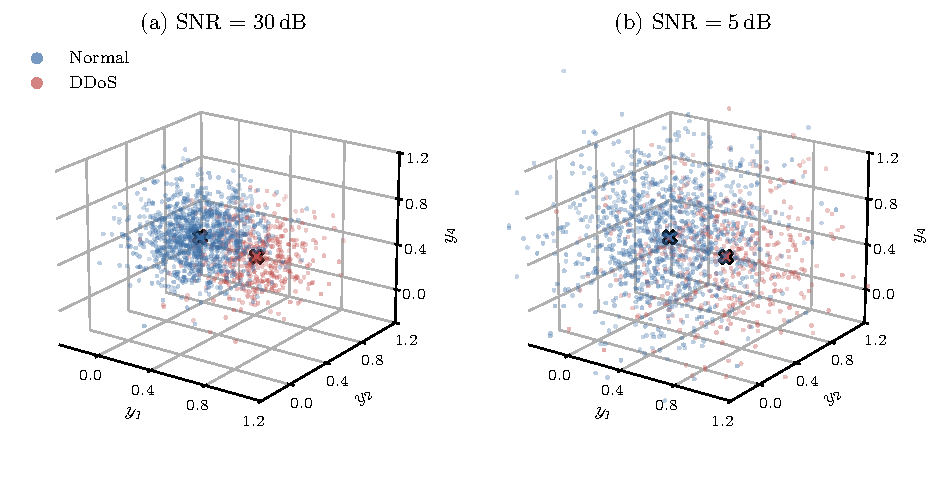
\includegraphics[width=\textwidth]{three_d_feature_space.pdf}
	\caption{Dreidimensionaler Ausschnitt des Merkmalsraums ($y_1$, $y_2$, $y_4$) für dieselben $1\,500$ Flüsse bei (a) $30$\,dB und (b) $5$\,dB. Blau: Normalverkehr, rot: DDoS, Kreuze: Klassenmittelwerte $\boldsymbol\mu_c$.}
	\label{fig:feature_raum_3d}
\end{figure}

Evaluiert werden $\mathrm{SNR}\in\{30,20,10,5\}$\,dB. Mehr zur technischen Umsetzung steht in Abschnitt~\ref{sec:gymnasium_umgebung} und~\ref{sec:awgn_kanal}.

\section{Umgang mit Klassenungleichgewichten (Imbalanced Data)}
\label{sec:imbalanced_data}

Ein wesentlicher methodischer Aspekt in der Erkennung von Netzwerkangriffen ist das Problem des Klassenungleichgewichts, auch als Imbalanced Data bezeichnet. In realen Netzwerken tritt der legitime Verkehr typischerweise deutlich häufiger auf als Angriffsverkehr, wodurch die Zielklassen in den Trainingsdaten stark asymmetrisch verteilt sind. Diese Verteilung ist in Sicherheitsanwendungen nicht nur statistisch relevant, sondern auch fachlich bedeutsam, da die Minderheitsklasse, also der bösartige Verkehr, häufig die operational entscheidenden Ereignisse repräsentiert. Ein Modell, das nur auf Gesamtgenauigkeit optimiert wird, kann daher eine hohe Gesamtleistung erzielen, zugleich aber die Erkennung von Angriffen vernachlässigen, weil die Mehrheitsklasse den Lernprozess dominiert.

Das Problem des Klassenungleichgewichts wirkt sich auf mehrere Ebenen aus. Zum einen entstehen im Training verzerrte Entscheidungsgrenzen, wenn der Algorithmus die Minderheitsklasse als wenig relevant behandelt. Zum anderen kann die Bewertung der Modelle durch klassische Metriken wie Accuracy irreführend werden, weil eine hohe Gesamtzahl korrekt klassifizierter Instanzen nicht zwingend einer guten Angriffserkennung entspricht. Gerade in einem Sicherheitskontext ist jedoch die Erkennung von tatsächlich vorhandenen Angriffen von hoher Bedeutung, da bereits ein einzelner unerkannter Angriff zu erheblichen Ausfallzeiten oder organisatorischen Schäden führen kann.

Für die Behandlung unbalancierter Datensätze stehen verschiedene Strategien zur Verfügung. Datenbasiert können Verfahren wie Oversampling, Undersampling oder synthetische Generierung von Minderheitsinstanzen angewendet werden, um die relative Repräsentation der Angriffs- und Normalverkehrsanteile anzupassen. Modellbasiert können zudem klassenspezifische Gewichte, kosten-sensitive Verlustfunktionen oder adaptierte Entscheidungsgrenzen eingesetzt werden, damit die Fehlklassifikation von Angriffen im Lernprozess stärker penalisiert wird. In dieser Arbeit liegt der Angriffsanteil bei $0{,}3$ und die Fehlerkosten werden über die Reward-Matrix gewichtet ($R_{FN}=-2$ gegenüber $R_{FP}=-1$), ohne Resampling. Eine methodisch saubere Anwendung von Resampling erfordert dabei, dass Resampling und Gewichtungen ausschließlich auf den Trainingsdaten erfolgen, um Datenleckage zu vermeiden und die spätere Evaluation auf repräsentativen Testdaten zu basieren.

Neben der Anpassung der Trainingsstrategie ist auch die Auswahl geeigneter Evaluationsmetriken von zentraler Bedeutung. Während Accuracy in unbalancierten Datensätzen nur eingeschränkt aussagekräftig ist, liefern Precision, Recall, F1-Score und im geeigneten Kontext auch ROC-AUC oder PR-AUC eine belastbarere Einschätzung der Erkennungsleistung. Diese Kennzahlen erlauben eine differenzierte Bewertung, ob ein Modell zwar viele legitime Verbindungen korrekt erkennt, aber zugleich die gefährlichsten Angriffsbeispiele verfehlt. Für die hier betrachtete Anwendung ist diese Unterscheidung von besonderer Bedeutung, da eine hohe Sensitivität bei der Angriffserkennung oft Vorrang vor einer rein hohen Gesamtgenauigkeit hat.

Insgesamt zeigt sich, dass die Behandlung von Klassenungleichgewichten nicht als isolierter Preprocessing-Schritt verstanden werden darf, sondern als integraler Bestandteil der gesamten Modell- und Evaluationspipeline. Erst durch eine konsistente Kombination aus geeigneter Datenrepräsentation, gezielter Feature-Auswahl, resampling-basierter Ausgewogenheit und aussagekräftiger Metrikbewertung lässt sich eine belastbare und praxisnahe Erkennung von Angriffen in realen Netzwerken erreichen. Dieses Kapitel bildet damit die methodische Grundlage für die anschließende Implementierung und die nachfolgenden experimentellen Evaluationen.

\chapter{Implementierung des DDQN-Ansatzes}
\label{chap:implementierung}

Dieses Kapitel beschreibt, wie der in Abschnitt~\ref{sec:ansatz_vergleich} gewählte Double-DQN-Agent (DDQN) in PyTorch umgesetzt ist. Die Implementierung besteht aus drei Teilen: einer Gymnasium-Umgebung, die Netzwerkflüsse als Merkmalsvektoren erzeugt und über einen AWGN-Kanal stört, dem DDQN-Agenten mit Replay-Puffer und Zielnetz sowie einer vektorisierten Trainingsschleife, die standardmäßig auf einer CUDA-GPU läuft. Alle Größen stammen aus dem Quelltext (\texttt{train\_eval.py}).

\section{Systemarchitektur und Gesamtüberblick}
\label{sec:systemarchitektur}

Jeder Netzwerkfluss ist eine eigene, unabhängige Entscheidung. Der Agent erhält einen verrauschten Merkmalsvektor, wählt \emph{Normal} oder \emph{DDoS} und bekommt sofort eine Belohnung. Der Folgefluss hängt weder von der Aktion noch vom aktuellen Fluss ab. Eine Episode umfasst deshalb genau einen Schritt (\texttt{terminated=True}). Die Pipeline lässt sich in vier Stufen gliedern:

\begin{enumerate}
	\item \textbf{Flussgenerator:} Aus dem Modell in Abschnitt~\ref{sec:generatormodell} entsteht pro Fluss ein Vektor $\mathbf{x}\in\mathbb{R}^8$ samt Label.
	\item \textbf{AWGN-Kanal:} Auf $\mathbf{x}$ wird additives Rauschen entsprechend dem SNR addiert, der Agent sieht $\mathbf{y}$.
	\item \textbf{DDQN-Agent:} Ein Q-Netz bewertet beide Aktionen, die Aktion mit dem größten Q-Wert (bzw. eine $\epsilon$-greedy-Aktion) wird ausgeführt.
	\item \textbf{Lernschritt:} Die Transition wird im Replay-Puffer gespeichert, aus dem Mini-Batches das Online-Netz trainieren.
\end{enumerate}

Abbildung~\ref{fig:blockschaltbild} zeigt die Wirkungskette vom Flussgenerator bis zur Entscheidung. Der Rückpfad vom Reward in den Replay-Puffer schließt den Lernkreis, der Reward erreicht den Agenten also ausschließlich als Trainingssignal und nie als Eingabe.

\begin{figure}[htbp]
	\centering
	\begin{tikzpicture}[
		font=\small,
		blk/.style={draw, rectangle, rounded corners=2pt, minimum height=1.35cm, text width=2.7cm, align=center, thick},
		ch/.style={blk, fill=blue!8, text width=3.0cm},
		ag/.style={blk, fill=green!10},
		rw/.style={blk, fill=orange!12, text width=3.0cm},
		sub/.style={draw, rectangle, minimum height=0.5cm, text width=2.4cm, align=center, font=\scriptsize, fill=white},
		arr/.style={-{Stealth[length=2.2mm]}, thick}
	]
		% Umgebung: Generator, Kanal, Reward
		\node[blk] (gen) at (0,0) {Flussgenerator\\ {\scriptsize $\mathbf{x}\in\mathbb{R}^{8}$, Label $c$}};
		\node[ch] (awgn) at (4.4,0) {AWGN-Kanal\\ {\scriptsize $\sigma_{n,j}^{2}=P_j/10^{\mathrm{SNR}/10}$\\ SNR $30$ bis $5$\,dB}};
		\node[rw] (rew) at (11.4,0) {Reward-Matrix\\ {\scriptsize asymmetrisch, $r(a,c)$}};
		\draw[arr] (gen) -- node[above, font=\scriptsize] {$\mathbf{x}$} (awgn);
		\draw[arr] (gen.north) -- ++(0,0.45) -| node[pos=0.25, above, font=\scriptsize] {Label $c$} (rew.north);
		\begin{scope}[on background layer]
			\node[draw=black!55, dashed, rounded corners=3pt, fit=(gen)(awgn)(rew), inner xsep=0.25cm, inner ysep=0.95cm, yshift=0.4cm,
				label={[font=\scriptsize, black!70, anchor=north west, inner sep=2pt]north west:Gymnasium-Umgebung \texttt{DDoSFlowEnv}}] (gym) {};
		\end{scope}

		% Agent mit Innenleben
		\node[ag] (agent) at (4.4,-3.3) {DDQN-Agent\\ {\scriptsize $\epsilon$-greedy}};
		\node[sub, below=0.3cm of agent] (onl) {Online-Netz $\theta$};
		\node[sub, below=0.1cm of onl] (tgt) {Zielnetz $\bar\theta$};
		\node[sub, below=0.1cm of tgt] (rb) {Replay-Puffer};
		\begin{scope}[on background layer]
			\node[draw, dashed, fit=(agent)(onl)(tgt)(rb), inner sep=4pt, fill=green!5] (agbox) {};
		\end{scope}

		% Entscheidung
		\node[blk] (dec) at (11.4,-3.3) {Entscheidung\\ {\scriptsize $a\in\{0,1\}$}};

		\draw[arr] (awgn) -- node[pos=0.72, right, font=\scriptsize] {Beobachtung $\mathbf{y}$} (agbox.north);
		\draw[arr] (agent) -- node[above, font=\scriptsize] {$a$} (dec);
		\draw[arr] (dec) -- node[right, font=\scriptsize] {$a$} (rew);
		\draw[arr, dashed] (rew.east) -- ++(0.45,0) |- node[pos=0.75, below, font=\scriptsize] {Reward $r$} (rb.east);
	\end{tikzpicture}
	\caption[Blockschaltbild der Wirkungskette]{Blockschaltbild der Wirkungskette. Die Gymnasium-Umgebung (gestrichelter Rahmen) erzeugt $\mathbf{x}$ mit Label $c$, stört $\mathbf{x}$ über den AWGN-Kanal und bewertet die Entscheidung $a$ des Agenten über die Reward-Matrix gegen $c$. Der Reward $r$ gelangt nur als Trainingssignal in den Replay-Puffer (gestrichelter Pfeil), nie als Eingabe des Agenten.}
	\label{fig:blockschaltbild}
\end{figure}

Der Zustand ist direkt der Merkmalsvektor, der Aktionsraum hat zwei Elemente. Diese Vereinfachung hält die Umgebung schnell: Der Flussgenerator erzeugt 32 Flüsse pro Iteration vektorisiert in NumPy, und Puffer, Netze und Rewards liegen auf demselben Rechengerät (standardmäßig eine CUDA-GPU), sodass beim Sampling kein Transfer zwischen Host und Gerät anfällt.

\section{Gymnasium-Umgebung und Zustandsraum}
\label{sec:gymnasium_umgebung}

Die Klasse \texttt{DDoSFlowEnv} erbt von \texttt{gymnasium.Env} und definiert:

\begin{itemize}
	\item \textbf{Beobachtungsraum:} \texttt{Box}$(-\infty,\infty)^{8}$ vom Typ \texttt{float32}, der verrauschte Merkmalsvektor $\mathbf{y}$.
	\item \textbf{Aktionsraum:} \texttt{Discrete}$(2)$ mit $a=0$ (Normal) und $a=1$ (DDoS).
	\item \textbf{Reset:} zieht einen neuen Fluss mit Label $c\in\{0,1\}$ (Angriffsanteil $\pi=0{,}3$) beim fest eingestellten SNR der Umgebung.
	\item \textbf{Step:} berechnet den Reward aus Aktion und Label, liefert eine Null-Beobachtung und setzt \texttt{terminated=True}. Die Terminal-Beobachtung geht nicht in das Lernen ein.
\end{itemize}

Der Gymnasium-Umgebungsprüfer (\texttt{check\_env}) validiert die Schnittstelle vor jedem Lauf. Die Belohnung hängt allein vom Zusammenspiel von Aktion und wahrem Label ab:

\begin{equation}
	r(a,c)=
	\begin{cases}
		R_{\mathrm{TP}}=+1{,}0, & a=1,\ c=1 \\
		R_{\mathrm{TN}}=+0{,}5, & a=0,\ c=0 \\
		R_{\mathrm{FP}}=-1{,}0, & a=1,\ c=0 \\
		R_{\mathrm{FN}}=-2{,}0, & a=0,\ c=1 .
	\end{cases}
\end{equation}

Ein verpasster Angriff kostet doppelt so viel wie ein Fehlalarm. Diese Asymmetrie wirkt als kostensensitives Lernziel anstelle eines Resamplings (Abschnitt~\ref{sec:imbalanced_data}). Für die Evaluation in Kapitel~\ref{chap:ergebnisse} hat sie eine konkrete Folge, nämlich die Verschiebung der Soll-Schwelle auf $p>1/3$ (Abschnitt~\ref{sec:mdp_definition}).

\subsection{Formale Definition als Markov-Entscheidungsprozess}
\label{sec:mdp_definition}

Das Entscheidungsproblem ist ein Markov-Entscheidungsprozess $(\mathcal{S},\mathcal{A},\mathcal{P},\mathcal{R},\gamma)$ in der Notation von Sutton und Barto \autocite{suttonReinforcementLearningIntroduction2018} mit folgenden Komponenten:

\begin{itemize}
	\item \textbf{Zustandsraum:} $\mathcal{S}=\mathbb{R}^{8}$. Ein Zustand ist die verrauschte Beobachtung $\mathbf{y}=\mathbf{x}+\mathbf{n}$ mit $n_j\sim\mathcal{N}(0,\sigma_{n,j}^2)$ aus Abschnitt~\ref{sec:awgn_kanal}. Das Label $c$ gehört nicht zum Zustand, der Prozess ist bezüglich $c$ nur teilbeobachtbar.
	\item \textbf{Aktionsraum:} $\mathcal{A}=\{0,1\}$, mit $a=0$ für Normalverkehr und $a=1$ für DDoS.
	\item \textbf{Transition:} $\mathcal{P}(\mathbf{y}'\mid\mathbf{y},a)$ ist deterministisch und von $(\mathbf{y},a)$ unabhängig. Jede Episode endet nach einem Schritt, das Terminal-Flag ist stets $d=1$:
	\begin{equation}
		\mathcal{P}(\mathbf{y}'\mid\mathbf{y},a)=\delta(\mathbf{y}'-\mathbf{0}),\qquad d=1 .
	\end{equation}
	Der Folgezustand ist die Null-Beobachtung aus \texttt{step}. Der nächste Fluss entsteht erst im \texttt{reset}. Im vektorisierten Training speichert der Replay-Puffer als Folgebeobachtung stattdessen die aktuelle Beobachtung $\mathbf{y}$. Wegen $d=1$ geht dieser Wert in keines der Lernziele ein.
	\item \textbf{Belohnung:} $\mathcal{R}(a,c)$ als Reward-Matrix mit Zeilen $c$ und Spalten $a$:
	\begin{equation}
		\mathcal{R}=
		\begin{pmatrix}
			\mathcal{R}(0,0) & \mathcal{R}(1,0)\\
			\mathcal{R}(0,1) & \mathcal{R}(1,1)
		\end{pmatrix}
		=
		\begin{pmatrix}
			R_{\mathrm{TN}} & R_{\mathrm{FP}}\\
			R_{\mathrm{FN}} & R_{\mathrm{TP}}
		\end{pmatrix}
		=
		\begin{pmatrix}
			+0{,}5 & -1{,}0\\
			-2{,}0 & +1{,}0
		\end{pmatrix}.
	\end{equation}
	Das entspricht \texttt{REWARD\_TABLE[label, action]} im Quelltext.
	\item \textbf{Diskontierung:} $\gamma=0{,}99$. Wegen $d=1$ geht $\gamma$ nicht in das Ziel ein.
\end{itemize}

Die optimale Politik maximiert den erwarteten Sofort-Reward $\mathbb{E}[\mathcal{R}(a,c)\mid\mathbf{y}]$. Mit $p=P(c=1\mid\mathbf{y})$ gilt $a=1$ genau dann, wenn $p\,R_{\mathrm{TP}}+(1-p)\,R_{\mathrm{FP}}>p\,R_{\mathrm{FN}}+(1-p)\,R_{\mathrm{TN}}$, also $p>1/3$. Elkans Schwelle $p^*=(c_{10}-c_{00})/(c_{10}-c_{00}+c_{01}-c_{11})$ liefert mit den negierten Rewards als Kosten denselben Wert \autocite{elkanFoundationsCostSensitiveLearning2001}. Das ist die Soll-Schwelle, wenn das Q-Netz die bedingten Erwartungswerte des Rewards lernt. Der im Training verwendete Huber-Verlust verschiebt sie auf $3/7$ (Abschnitt~\ref{sec:dqn_architektur}), gemessen entscheidet der Agent bei impliziten Schwellen von $0{,}38$ bis $0{,}43$ (Abschnitt~\ref{sec:reward_recall}).

Im Training werden die Flüsse nicht einzeln über \texttt{step} erzeugt, sondern als Batch von 32 Flüssen pro Iteration, wobei das SNR jedes Flusses zufällig aus $\{30,20,10,5\}$\,dB gezogen wird. Der Rewardvektor entsteht durch eine Tabellenabfrage \texttt{REWARD\_TABLE[label, action]} direkt auf dem Rechengerät.

\section{DDQN-Architektur in PyTorch}
\label{sec:dqn_architektur}

Das Q-Netz (\texttt{QNet}) ist ein vollständig verbundenes Netz mit zwei verdeckten Schichten:
\begin{equation}
	\mathbb{R}^{8}\ \to\ \underbrace{128}_{\text{ReLU}}\ \to\ \underbrace{128}_{\text{ReLU}}\ \to\ \mathbb{R}^{2}.
\end{equation}
Abbildung~\ref{fig:qnet_architektur} stellt die Struktur dar. Mit Gewichtsmatrizen $\mathbf{W}_1\in\mathbb{R}^{128\times8}$, $\mathbf{W}_2\in\mathbb{R}^{128\times128}$, $\mathbf{W}_3\in\mathbb{R}^{2\times128}$ und Biasvektoren $\mathbf{b}_i$ berechnet das Netz
\begin{equation}
	\mathbf{q}(\mathbf{y})=\mathbf{W}_3\,\mathrm{ReLU}\!\bigl(\mathbf{W}_2\,\mathrm{ReLU}(\mathbf{W}_1\mathbf{y}+\mathbf{b}_1)+\mathbf{b}_2\bigr)+\mathbf{b}_3 .
\end{equation}
Die Parameterzahl beträgt $(8\cdot128+128)+(128\cdot128+128)+(128\cdot2+2)=17\,922$ je Netz.

\begin{figure}[htbp]
	\centering
	\begin{tikzpicture}[
		font=\small,
		lay/.style={draw, rectangle, rounded corners=2pt, minimum height=2.2cm, minimum width=1.5cm, align=center, thick},
		arr/.style={-{Stealth[length=2.2mm]}, thick},
		node distance=1.3cm
	]
		\node[lay, fill=gray!10] (in) {Eingabe\\ $\mathbf{y}\in\mathbb{R}^{8}$};
		\node[lay, fill=blue!10, right=of in] (h1) {Linear\\ $8\to128$\\ ReLU};
		\node[lay, fill=blue!10, right=of h1] (h2) {Linear\\ $128\to128$\\ ReLU};
		\node[lay, fill=green!10, right=of h2] (out) {Linear\\ $128\to2$};
		\node[right=1.0cm of out, align=left] (q) {$Q(\mathbf{y},0)$\\[2pt] $Q(\mathbf{y},1)$};
		\draw[arr] (in) -- (h1);
		\draw[arr] (h1) -- (h2);
		\draw[arr] (h2) -- (out);
		\draw[arr] (out) -- (q);
	\end{tikzpicture}
	\caption[Feedforward-Struktur des Q-Netzes]{Feedforward-Struktur des Q-Netzes ($8\to128\to128\to2$, ReLU in beiden verdeckten Schichten, lineare Ausgabe). Online- und Zielnetz teilen sich diese Struktur.}
	\label{fig:qnet_architektur}
\end{figure}

Die Ausgabeschicht ist linear, die zwei Ausgaben sind die Q-Werte $Q(\mathbf{y},0)$ und $Q(\mathbf{y},1)$. Online-Netz und Zielnetz haben dieselbe Struktur, das Zielnetz startet mit den Gewichten des Online-Netzes und wird nur kopiert, nie per Gradient trainiert. Zielnetz und Replay-Puffer gehen auf den DQN-Ansatz von Mnih et al. zurück, wo sie die Korrelation aufeinanderfolgender Transitionen aufbrechen und das Regressionsziel zwischen zwei Synchronisationen festhalten \autocite{mnihHumanlevelControlDeep2015}.

Im Standard-DQN wählt und bewertet dasselbe Zielnetz die Folgeaktion:
\begin{equation}
	Y^{\mathrm{DQN}} = r + \gamma\,(1-d)\,\max_{a'} Q(\mathbf{y}',a';\bar{\theta}).
\end{equation}
Sind die Q-Schätzungen verrauscht, greift der $\max$-Operator bevorzugt Aktionen mit positivem Schätzfehler heraus, und das Ziel überschätzt den wahren Wert systematisch. Das DDQN-Ziel nach van Hasselt et al. trennt deshalb Aktionsauswahl und Bewertung \autocite{vanhasseltDeepReinforcementLearning2016}:
\begin{equation}
	Y = r + \gamma\,(1-d)\;Q\!\left(\mathbf{y}',\ \arg\max_{a'} Q(\mathbf{y}',a';\theta);\ \bar{\theta}\right),
\end{equation}
wobei $\theta$ die Parameter des Online-Netzes, $\bar\theta$ die des Zielnetzes und $d\in\{0,1\}$ das Terminal-Flag sind. Der Verlust ist die Huber-Funktion (\texttt{smooth\_l1\_loss}) zwischen $Q(\mathbf{y},a;\theta)$ und $Y$, die Gradientennorm wird auf $10$ begrenzt.

Weil jede Episode nach einem Schritt endet, gilt für alle gespeicherten Transitionen $d=1$ und damit $Y=r$. Abbildung~\ref{fig:backup} stellt den allgemeinen Fall und diesen Spezialfall als Backup-Diagramme gegenüber. Das Bootstrapping-Glied entfällt, der Diskontierungsfaktor $\gamma$ beeinflusst das Lernen nicht, und das Q-Netz regressiert den Sofort-Reward je Aktion (ein kontextuelles Banditenproblem). Online-/Zielnetz, Double-Q-Ziel und Replay-Puffer sind vollständig implementiert und bleiben im Code aktiv. Unter diesem Problemzuschnitt geht das Zielnetz wegen $d=1$ jedoch nie in $Y$ ein. Die Überschätzung, gegen die van Hasselt et al. das Double-Q-Ziel entwickelt haben, entsteht erst im Bootstrapping-Glied und kann hier nicht auftreten. Wirksam bleiben der Replay-Puffer, der die Mini-Batches dekorreliert, und die Huber-Regression auf den Sofort-Reward. Das ist bei der Interpretation der Ergebnisse zu berücksichtigen.

Der Huber-Verlust hat dabei eine Nebenwirkung auf die Entscheidungsschwelle. Er ist für Residuen $|Y-Q|\le1$ quadratisch und darüber linear. Die Rewards einer Aktion liegen aber $2$ (Aktion DDoS: $+1$ oder $-1$) bzw. $2{,}5$ (Aktion Normal: $-2$ oder $+0{,}5$) auseinander. Das Minimum des erwarteten Verlusts liegt deshalb nicht beim bedingten Erwartungswert, sondern zwischen Erwartungswert und Median. Für $p<1/2$ ergibt die Stationaritätsbedingung $Q_{\mathrm{H}}(\mathbf{y},1)=(2p-1)/(1-p)$ und $Q_{\mathrm{H}}(\mathbf{y},0)=0{,}5-p/(1-p)$, für $p>1/2$ entsprechend $(2p-1)/p$ und $(1-p)/p-2$. Daraus folgt
\begin{equation}
	Q_{\mathrm{H}}(\mathbf{y},1)-Q_{\mathrm{H}}(\mathbf{y},0)=
	\begin{cases}
		\dfrac{3{,}5\,p-1{,}5}{1-p}, & p<1/2,\\[8pt]
		\dfrac{5\,p-2}{p}, & p>1/2,
	\end{cases}
\end{equation}
mit der Nullstelle $p=3/7\approx0{,}43$ statt $1/3$. Ein mit diesem Verlust trainiertes Q-Netz entscheidet also konservativer, als die Reward-Matrix vorgibt. Abschnitt~\ref{sec:reward_recall} prüft das am trainierten Netz.

\begin{figure}[htbp]
	\centering
	\begin{tikzpicture}[
		font=\small,
		st/.style={circle, draw, thick, minimum size=4.4mm, inner sep=0pt},
		ac/.style={circle, fill, minimum size=2.3mm, inner sep=0pt},
		te/.style={rectangle, fill, minimum size=2.8mm, inner sep=0pt},
		gst/.style={circle, draw=black!35, dashed, thick, minimum size=4.4mm, inner sep=0pt},
		gac/.style={circle, fill=black!30, minimum size=2.3mm, inner sep=0pt},
		ed/.style={thick},
		ged/.style={draw=black!35, dashed, thick}
	]
		% (a) allgemeiner Fall
		\begin{scope}
			\node[ac, label={[font=\scriptsize]above:$(s,a)$}] (sa) at (0,0) {};
			\node[st] (s1) at (0,-1.25) {};
			\node[font=\scriptsize, right=1.5mm of s1] {$s'$};
			\draw[ed] (sa) -- node[left, font=\scriptsize] {$r$} (s1);
			\foreach \x/\n in {-0.75/a1, 0/a2, 0.75/a3} { \node[ac] (\n) at (\x,-2.45) {}; \draw[ed] (s1) -- (\n); }
			\draw[thick] ($(s1)!0.42!(a1)$) to[bend right=35] ($(s1)!0.42!(a3)$);
			\node[font=\scriptsize, anchor=east] at ($(s1)!0.42!(a1)+(-0.05,0)$) {$\max$};
			\node[font=\scriptsize, below=1mm of a2] {$a'$};
			\node[font=\scriptsize, right=1.5mm of a3, align=left] {wählt: Online-Netz $\theta$\\ bewertet: Zielnetz $\bar\theta$};
			\node[font=\scriptsize] at (0.6,-3.3) {$Y=r+\gamma\,(1-d)\,Q\bigl(s',\arg\max_{a'}Q(s',a';\theta);\bar\theta\bigr)$};
			\node at (0.6,-3.95) {(a) allgemeiner Fall ($d=0$)};
		\end{scope}
		% (b) Ein-Schritt-Episode dieser Arbeit
		\begin{scope}[xshift=8.4cm]
			\node[ac, label={[font=\scriptsize]above:$(\mathbf{y},a)$}] (ya) at (0,0) {};
			\node[te] (T) at (0,-1.25) {};
			\node[font=\scriptsize, right=1.5mm of T] {Terminalzustand, $d=1$};
			\draw[ed] (ya) -- node[left, font=\scriptsize] {$r$} (T);
			\node[gst] (g1) at (0,-1.95) {};
			\draw[ged] (T) -- (g1);
			\foreach \x/\n in {-0.6/b1, 0/b2, 0.6/b3} { \node[gac] (\n) at (\x,-2.75) {}; \draw[ged] (g1) -- (\n); }
			\node[font=\scriptsize, text=black!55, right=1.5mm of b3, align=left] {Bootstrapping-Zweig\\ entfällt: $\gamma\,(1-d)=0$};
			\node[font=\scriptsize] at (0.6,-3.3) {$Y=r$};
			\node at (0.6,-3.95) {(b) diese Arbeit (Ein-Schritt-Episode)};
		\end{scope}
	\end{tikzpicture}
	\caption[Backup-Diagramme des Lernziels]{Backup-Diagramme des Lernziels in der Notation von Sutton und Barto \autocite{suttonReinforcementLearningIntroduction2018} (offener Kreis: Zustand, Punkt: Aktion, Quadrat: Terminalzustand). (a) Im allgemeinen Fall bootstrappt das Double-DQN-Ziel über den Folgezustand $s'$: Das Online-Netz wählt $a'$, das Zielnetz bewertet sie. (b) In dieser Arbeit endet jede Episode nach einem Schritt. Der Bootstrapping-Zweig (grau) entfällt, das Ziel reduziert sich auf $Y=r$, und Zielnetz und Double-Q-Ziel gehen nicht in das Lernen ein.}
	\label{fig:backup}
\end{figure}

Der Replay-Puffer (\texttt{ReplayBuffer}) ist ein Ringpuffer mit $50\,000$ Einträgen nach dem Schema von Mnih et al. \autocite{mnihHumanlevelControlDeep2015}. Er hält Beobachtung, Aktion, Reward, Folgebeobachtung und Terminal-Flag als Tensoren auf dem Zielgerät und zieht gleichverteilte Mini-Batches der Größe $64$.

\section{AWGN-Kanalmodell im Lernprozess}
\label{sec:awgn_kanal}

Der Agent beobachtet $\mathbf{y}=\mathbf{x}+\mathbf{n}$ mit $n_j\sim\mathcal{N}(0,\sigma_{n,j}^2)$ je Merkmal $j$. Das ist das AWGN-Kanalmodell der Nachrichtentechnik \autocite{proakisDigitalCommunications2008}, hier nicht auf ein Sendesignal, sondern auf den Merkmalsvektor angewendet (Abschnitt~\ref{sec:merkmalsrauschen}). Die Rauschvarianz richtet sich nach der Signalleistung $P_j=\mathbb{E}[x_j^2]$ des Merkmals und dem gewünschten SNR (Abschnitt~\ref{sec:generatormodell}):
\begin{equation}
	\sigma_{n,j}^2=\frac{P_j}{10^{\mathrm{SNR_{dB}}/10}}.
\end{equation}
Der Kanalfaktor ist $h=1$, es gibt keine Verstärkung oder Fading-Komponente. Bei $30$\,dB beträgt die Rauschvarianz $10^{-3}P_j$, bei $5$\,dB etwa $0{,}32\,P_j$. Die Rauschstandardabweichung beträgt damit etwa $3\,\%$ (bei $30$\,dB) bis $56\,\%$ (bei $5$\,dB) von $\sqrt{P_j}$. Bei $5$\,dB liegt die Rauschstandardabweichung mit $0{,}22$ bis $0{,}31$ je Merkmal über der intrinsischen Klassenstreuung $\sigma=0{,}20$.

\subsection{Klassenüberlappung bei sinkendem SNR}
\label{sec:klassenueberlappung}

Das Rauschen verbreitert beide Klassenverteilungen. Die Beobachtung ist klassenbedingt wieder gaußverteilt, denn die Summe zweier unabhängiger Gauß-Terme bleibt gaußförmig:
\begin{equation}
	y_j\mid c\sim\mathcal{N}\!\bigl(\mu_{c,j},\ \sigma^2+\sigma_{n,j}^2\bigr).
\end{equation}
Die Klassenmittelwerte bleiben fest, nur die Varianz wächst von $\sigma^2=0{,}04$ auf $\sigma^2+\sigma_{n,j}^2$. Der Abstand der Mittelwerte $\Delta\mu_j=\mu_{\text{DDoS},j}-\mu_{\text{Normal},j}$ beträgt $\pm0{,}15$ bis $\pm0{,}25$. Bei gleicher Kovarianz beider Klassen (diagonal) ergibt sich der Mahalanobis-Abstand
\begin{equation}
	D^{2}=\sum_{j=1}^{8}\frac{\Delta\mu_j^{2}}{\sigma^{2}+\sigma_{n,j}^{2}},
\end{equation}
und die Bayes-Fehlerwahrscheinlichkeit für gleiche Priors ist $P_e=Q_{\mathrm{G}}(D/2)$ mit der Gaußschen Q-Funktion
\begin{equation}
	Q_{\mathrm{G}}(z)=\frac{1}{\sqrt{2\pi}}\int_{z}^{\infty}e^{-t^{2}/2}\,\mathrm{d}t .
\end{equation}
Der Index G trennt sie von der Aktionswertfunktion $Q(\mathbf{y},a)$ des Agenten. Der Zusammenhang entspricht der Symbolfehlerwahrscheinlichkeit binärer Signale im AWGN-Kanal, bei der $D$ die Rolle des normierten Signalabstands übernimmt \autocite{proakisDigitalCommunications2008}. Mit dem tatsächlichen Angriffsanteil $\pi=0{,}3$ verschiebt die Bayes-Regel ihre Schwelle um $\lambda=\ln\bigl((1-\pi)/\pi\bigr)$ auf der Skala des Log-Likelihood-Verhältnisses, und die minimale Fehlerwahrscheinlichkeit lautet
\begin{equation}
	P_e^{\pi}=\pi\,Q_{\mathrm{G}}\!\left(\frac{D}{2}-\frac{\lambda}{D}\right)+(1-\pi)\,Q_{\mathrm{G}}\!\left(\frac{D}{2}+\frac{\lambda}{D}\right).
\end{equation}
Für die Parameter aus \texttt{train\_eval.py} liefert die Auswertung die Werte in Tabelle~\ref{tab:klassenueberlappung}.

\begin{table}[htbp]
	\centering
	\renewcommand{\arraystretch}{1.25}
	\caption[Klassenseparierbarkeit der Beobachtung in Abhängigkeit vom SNR]{Klassenseparierbarkeit der Beobachtung $\mathbf{y}$ in Abhängigkeit vom SNR ($\sigma=0{,}20$). $P_e$: Bayes-Fehler bei gleichen Priors, $P_e^{\pi}$: Bayes-Fehler beim tatsächlichen Angriffsanteil $\pi=0{,}3$.}
	\label{tab:klassenueberlappung}
	\begin{tabular}{rrrrrr}
		\toprule
		\textbf{SNR in dB} & $\max_j\sigma_{n,j}$ & $D^{2}$ & $D$ & $P_e=Q_{\mathrm{G}}(D/2)$ & $P_e^{\pi}$ \\
		\midrule
		$30$ & $0{,}018$ & $8{,}76$ & $2{,}96$ & $6{,}9\,\%$ & $6{,}2\,\%$ \\
		$20$ & $0{,}056$ & $8{,}33$ & $2{,}89$ & $7{,}4\,\%$ & $6{,}6\,\%$ \\
		$10$ & $0{,}176$ & $5{,}62$ & $2{,}37$ & $11{,}8\,\%$ & $10{,}4\,\%$ \\
		$5$  & $0{,}312$ & $3{,}17$ & $1{,}78$ & $18{,}7\,\%$ & $16{,}2\,\%$ \\
		\bottomrule
	\end{tabular}
\end{table}

Zwischen $30$ und $20$\,dB ändert sich die Überlappung kaum, weil das Rauschen ($\sigma_{n,j}\le0{,}056$) neben $\sigma=0{,}20$ vernachlässigbar bleibt. Bei $5$\,dB sinkt $D$ auf $1{,}78$, die effektive Streuung steigt je nach Merkmal auf $0{,}30$ bis $0{,}37$, und die Fehlerwahrscheinlichkeit des Bayes-Klassifikators steigt gegenüber $30$\,dB auf fast das Dreifache. Beim tatsächlichen Angriffsanteil $\pi=0{,}3$ liegt sie auf jeder Stufe etwas niedriger, von $6{,}2\,\%$ bei $30$\,dB bis $16{,}2\,\%$ bei $5$\,dB. Diese Spalte ist die Referenz für alle weiteren Vergleiche mit der Bayes-Grenze. Das Training mit gemischtem SNR zwingt das Q-Netz auf eine Kompromiss-Entscheidungsgrenze, die für kein SNR exakt optimal ist.

Abbildung~\ref{fig:llr_signalraum} zeigt dieselbe Rechnung als Signalraumdarstellung auf der Prüfgröße $\Lambda(\mathbf{y})=\ln\bigl(p(\mathbf{y}\mid\mathrm{DDoS})/p(\mathbf{y}\mid\mathrm{Normal})\bigr)$. Sie bündelt wie bei binären Signalen im AWGN-Kanal die gesamte Klasseninformation der acht Merkmale \autocite{proakisDigitalCommunications2008}. Bei der fehlerminimalen Schwelle $\tau(1/2)=\lambda$ ergeben beide Fehlerflächen zusammen genau $P_e^{\pi}$: bei $30$\,dB $3{,}5\,\%$ verpasste Angriffe und $2{,}7\,\%$ Fehlalarme, bei $5$\,dB $10{,}2$ und $6{,}0\,\%$, jeweils bezogen auf alle Flüsse. Die Soll-Schwelle $p>1/3$ der Reward-Matrix liegt um $\ln 2\approx0{,}69$ weiter links und tauscht verpasste Angriffe gegen Fehlalarme. Bei $5$\,dB sinkt der FN-Anteil auf $6{,}3\,\%$, der FP-Anteil steigt auf $11{,}5\,\%$. Der Gesamtfehler wächst dabei von $16{,}2$ auf $17{,}8\,\%$, die erwarteten Kosten unter der Reward-Matrix sinken.

\begin{figure}[htbp]
	\centering
	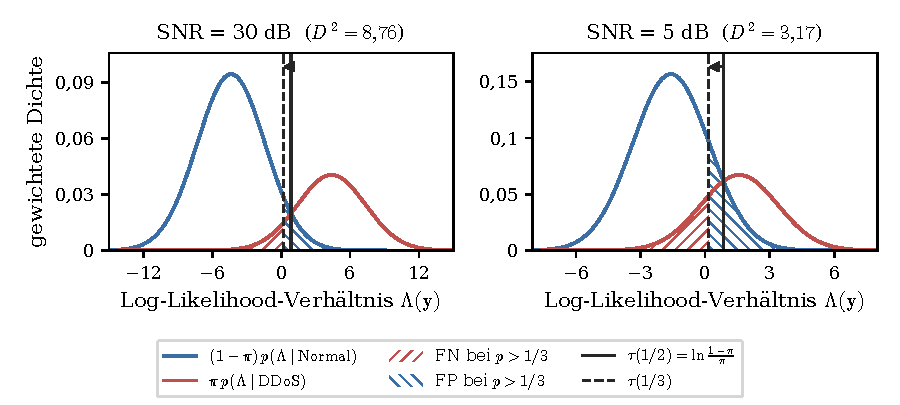
\includegraphics[width=\textwidth]{llr_signalraum_plot.pdf}
	\caption[Signalraumdarstellung auf dem Log-Likelihood-Verhältnis]{Signalraumdarstellung der binären Entscheidung auf der Prüfgröße $\Lambda(\mathbf{y})$ bei $30$ und $5$\,dB ($\pi=0{,}3$). Kurven: mit den Priors gewichtete Klassendichten $\pi\,\mathcal{N}(+D^2/2,D^2)$ und $(1-\pi)\,\mathcal{N}(-D^2/2,D^2)$. Durchgezogen: fehlerminimale Schwelle $\tau(1/2)=\lambda$, gestrichelt: Soll-Schwelle $\tau(1/3)$ der Reward-Matrix, Pfeil: Verschiebung um $\ln 2$. Schraffiert: Anteile verpasster Angriffe (FN) und Fehlalarme (FP) bei $p>1/3$.}
	\label{fig:llr_signalraum}
\end{figure}

Im Training trifft der Agent pro Fluss auf ein zufällig gewähltes SNR. Er lernt dadurch eine einzige Entscheidungsfunktion für alle vier Kanalqualitäten, ohne das SNR als Eingabe zu erhalten. Die Evaluation erfolgt dagegen getrennt je SNR-Stufe (Kapitel~\ref{chap:evaluierung}).

Das gemischte Training hat einen zweiten Effekt. Nach Bishop wirkt additives Eingangsrauschen im Training wie ein Tikhonov-Strafterm auf die Ableitungen der gelernten Abbildung (Abschnitt~\ref{sec:merkmalsrauschen}) \autocite{bishopTrainingNoiseEquivalent1995}. Das Q-Netz wird also gezwungen, $Q(\mathbf{y},a)$ glatt über $\mathbf{y}$ zu halten, und reagiert im Test weniger empfindlich auf einzelne Rauschausreißer. Apruzzese et al. nutzen dasselbe Prinzip mit gezielt gestörten Flussmerkmalen, um Detektoren gegen Evasion zu härten \autocite{apruzzeseDeepReinforcementAdversarial2020}. Streng gilt Bishops Äquivalenz nur für kleine Rauschvarianz. Bei $30$ und $20$\,dB ist diese Bedingung erfüllt ($\sigma_{n,j}\le0{,}056$), bei $5$\,dB mit $\sigma_{n,j}$ bis $0{,}31$ nicht mehr. Auf dieser Stufe bleibt die Regularisierungsdeutung eine qualitative Erklärung.

\section{Trainings- und Optimierungsstrategie}
\label{sec:training_optimierung}

Das Training läuft über $20\,000$ Iterationen. In jeder Iteration entstehen $32$ Flüsse, der Agent wählt $\epsilon$-greedy Aktionen, die Transitionen gelangen in den Puffer, und es folgt ein Lernschritt, sobald der Puffer mindestens $1000$ Einträge enthält. Die Explorationsrate fällt linear von $1{,}0$ auf $0{,}02$ innerhalb der ersten $40\,\%$ der Iterationen ($8000$) und bleibt danach konstant. Der Optimierer ist Adam mit Lernrate $10^{-4}$, der die Schrittweite je Gewicht aus gleitenden Schätzungen des ersten und zweiten Gradientenmoments anpasst \autocite{kingmaAdamMethodStochastic2015}. Das Zielnetz wird alle $250$ Lernschritte hart synchronisiert. Weil der Puffer je Iteration $32$ Transitionen aufnimmt, erreicht er die Mindestfüllung in Iteration $32$. Über den gesamten Lauf führt der Agent damit $19\,969$ Lernschritte mit je $64$ Transitionen aus und synchronisiert das Zielnetz $79$-mal. Ab Iteration $1563$ ist der Puffer voll, und neue Transitionen überschreiben die ältesten. Pro Seed (0, 1, 2) beginnt der Lauf mit neu initialisierten Netzen und eigenem Zufallsgenerator für die Flüsse. Die Seeds setzen Python-, NumPy- und PyTorch-Generatoren (inklusive CUDA).

\section{Implementierung in der praktischen Pipeline}
\label{sec:praktische_pipeline}

Das Skript \texttt{train\_eval.py} führt für jeden Seed Training und Evaluation aus und schreibt \texttt{evaluation\_results.csv} mit Precision, Recall und F1-Score je Seed und SNR sowie Mittelwert und Standardabweichung. Die Baselines (Random Forest, SVM, MLP) laufen in \texttt{eval\_baselines.py} und importieren Flussgenerator und Kanalmodell unverändert aus \texttt{train\_eval.py}. Dadurch sehen alle Verfahren dieselbe Datenverteilung und exakt dieselben Testflüsse. Die Abbildungen entstehen in \texttt{generate\_plot.py} aus den beiden CSV-Dateien.

Tabelle~\ref{tab:dqn_hyperparameters} fasst die Hyperparameter zusammen, Tabelle~\ref{tab:system_parameters} die Umgebungs- und Kanalparameter.

\begin{table}[htbp]
	\centering
	\renewcommand{\arraystretch}{1.25}
	\caption{Hyperparameter des DDQN-Agenten.}
	\label{tab:dqn_hyperparameters}
	\begin{tabular}{llL{6.2cm}}
		\toprule
		\textbf{Hyperparameter} & \textbf{Wert} & \textbf{Beschreibung} \\
		\midrule
		Netzstruktur & $8\to128\to128\to2$ & Zwei verdeckte Schichten mit ReLU \\
		Lernrate & $1\cdot10^{-4}$ & Adam-Optimierer \\
		Diskontierungsfaktor $\gamma$ & $0{,}99$ & Ohne Wirkung, da alle Episoden nach einem Schritt enden \\
		Batch-Größe & $64$ & Stichprobe pro Lernschritt \\
		Puffergröße & $50\,000$ & Ringpuffer auf dem Rechengerät \\
		Explorationsrate $\epsilon$ & $1{,}0 \to 0{,}02$ & Linear über $40\,\%$ der Iterationen \\
		Lernstart & $1000$ Einträge & Mindestfüllung des Puffers \\
		Zielnetz-Update & alle $250$ Lernschritte & Harte Synchronisation \\
		Verlustfunktion & Huber & Gradientennorm begrenzt auf $10$ \\
		Iterationen & $20\,000$ & Je $32$ Flüsse, insgesamt $6{,}4\cdot10^{5}$ Flüsse \\
		\bottomrule
	\end{tabular}

	\bigskip
	\renewcommand{\arraystretch}{1.25}
	\caption{System- und Kanalparameter der Simulationsumgebung.}
	\label{tab:system_parameters}
	\begin{tabular}{L{4.4cm}L{3.6cm}L{5.0cm}}
		\toprule
		\textbf{Parameter} & \textbf{Wert} & \textbf{Bedeutung} \\
		\midrule
		Zustandsraum & $\mathbb{R}^{8}$ & Verrauschter Merkmalsvektor $\mathbf{y}$ \\
		Aktionsraum & $2$ diskrete Aktionen & Normal (0), DDoS (1) \\
		Klassenstreuung $\sigma$ & $0{,}20$ & Je Merkmal, klassenbedingt gaußverteilt \\
		Angriffsanteil $\pi$ & $0{,}3$ & Klassenungleichgewicht \\
		Kanalmodell & AWGN, $h=1$ & Varianz $P_j/10^{\mathrm{SNR}/10}$ je Merkmal \\
		Evaluierte SNR-Werte & $30,\,20,\,10,\,5$\,dB & Abstufungen der Kanalqualität \\
		Reward\newline $(R_{\mathrm{TP}},R_{\mathrm{TN}},R_{\mathrm{FP}},R_{\mathrm{FN}})$ & $(+1;\,+0{,}5;\,-1;\,-2)$ & Asymmetrisch zulasten verpasster Angriffe \\
		Seeds & $0,\,1,\,2$ & Je ein vollständiger Trainings- und Testlauf \\
		Testflüsse & $20\,000$ je SNR und Seed & Frisch erzeugt, nicht im Training \\
		\bottomrule
	\end{tabular}
\end{table}

\section{Zusammenfassung der Implementierung}
\label{sec:implementierung_zusammenfassung}

Die Implementierung bildet die DDoS-Erkennung als Entscheidungsproblem mit acht verrauschten Merkmalen und zwei Aktionen ab, dessen Episoden nach einem Schritt enden. Das DDQN-Gerüst aus Online-Netz, Zielnetz, Double-Q-Ziel und Replay-Puffer ist vollständig umgesetzt. Die Kosten der Fehlerarten stecken in der Reward-Matrix, die Kanalqualität im AWGN-Modell mit SNR-Werten von $30$ bis $5$\,dB. Weil die Entscheidungen unabhängig sind, reduziert sich das Lernziel auf eine Huber-Regression des Sofort-Rewards. Kapitel~\ref{chap:ergebnisse} wertet die Läufe quantitativ aus.

\chapter{Evaluationsaufbau und Metriken}
\label{chap:evaluierung}

Dieses Kapitel legt fest, wie der in Kapitel~\ref{chap:implementierung} beschriebene Double-DQN-Agent (DDQN) bewertet wird. Es definiert das Evaluationsprotokoll, die Testbedingungen unter AWGN-Rauschen bei $\mathrm{SNR}\in\{30,20,10,5\}$\,dB, die Vergleichsmodelle und die Bewertungsmetriken Precision, Recall und F1-Score. Die Messergebnisse folgen in Kapitel~\ref{chap:ergebnisse}.

\section{Evaluationsprotokoll und Versuchsaufbau}
\label{sec:eval_protokoll}

Die Evaluation folgt einem reproduzierbaren zweistufigen Protokoll aus Training und Test. Einen separaten Validierungs-Split gibt es nicht: Die Hyperparameter in Tabelle~\ref{tab:dqn_hyperparameters} wurden vorab festgelegt und nicht anhand von Validierungsdaten nachgestellt. Die Datenbasis folgt dem Flussmodell aus Kapitel~\ref{chap:datensatz}. Der DDQN-Agent wurde in der in Abschnitt~\ref{sec:dqn_architektur} beschriebenen Konfiguration trainiert, wobei der SNR jedes Trainingsflusses zufällig aus $\{30,20,10,5\}$\,dB gezogen wurde (Abschnitt~\ref{sec:awgn_kanal}). Der Test erfolgt für jede SNR-Stufe getrennt auf 20\,000 frisch erzeugten Flüssen, die ein eigener Zufallsgenerator liefert und die im Training nie auftraten. Um die Abhängigkeit von einzelnen Initialisierungen zu reduzieren, wurde das Protokoll für die Seeds $0$, $1$ und $2$ mit identischer Hyperparameterkonfiguration durchlaufen und über die Seeds gemittelt.

Abbildung~\ref{fig:eval_protokoll} stellt den Ablauf dar. Trainings- und Testflüsse stammen aus getrennten Zufallsgeneratoren, das Training mischt die SNR-Stufen, der Test isoliert sie.

\begin{figure}[htbp]
	\centering
	\begin{tikzpicture}[
		font=\small,
		blk/.style={draw, rectangle, rounded corners=2pt, minimum height=1.1cm, text width=3.6cm, align=center, thick},
		arr/.style={-{Stealth[length=2.2mm]}, thick},
		node distance=0.7cm
	]
		% Training
		\node[blk, fill=blue!8] (trn) {Training mit gemischtem SNR\\ je Fluss $\mathrm{SNR}\sim\mathcal{U}\{30,20,10,5\}$\,dB};
		\node[blk, below=of trn] (ddqn) {DDQN\\ $20\,000\times32$ Flüsse, Reward-Signal};
		\node[blk, below=of ddqn] (base) {RF, SVM, MLP\\ $20\,000$ Flüsse, Labels};
		\draw[arr] (trn) -- (ddqn);
		\draw[arr] (ddqn) -- (base);
		% Test
		\node[blk, fill=green!10, right=3.2cm of trn] (tst) {Je SNR $\in\{30,20,10,5\}$\,dB isoliert};
		\node[blk, below=of tst] (flows) {$20\,000$ frische Flüsse\\ RNG-Seed $=1\,000\,003\,s+\mathrm{SNR}$};
		\node[blk, below=of flows] (pred) {Greedy-Entscheidung bzw. \texttt{predict}\\ $\to$ TP, FP, FN};
		\node[blk, below=of pred] (met) {Precision, Recall, F1\\ Mittel $\pm$ Std über Seeds $0,1,2$};
		\draw[arr] (tst) -- (flows);
		\draw[arr] (flows) -- (pred);
		\draw[arr] (pred) -- (met);
		\coordinate (join) at ($(ddqn.east)+(1.1,0)$);
		\draw (ddqn.east) -- (join);
		\draw (base.east) -| (join);
		\draw[arr] (join) |- (pred.west);
		\node[font=\scriptsize, above] at ($(ddqn.east)+(0.55,0)$) {Modelle};
		\node[above=0.15cm of trn, font=\scriptsize\bfseries] {Trainingsphase};
		\node[above=0.15cm of tst, font=\scriptsize\bfseries] {Testphase (keine Überschneidung)};
	\end{tikzpicture}
	\caption{Evaluationsprotokoll. Links: Training aller Modelle mit pro Fluss gemischtem SNR. Rechts: getrennte Testauswertung je SNR-Stufe auf $20\,000$ frischen Flüssen, wiederholt für drei Seeds. Die trainierten Modelle (DDQN, RF, SVM, MLP) laufen über denselben Testpfad und sehen identische Testflüsse.}
	\label{fig:eval_protokoll}
\end{figure}

Das Evaluationsszenario umfasst zwei komplementare Blickwinkel:

\begin{itemize}
	\item \textbf{Nominalbedingung}: Bewertung unter hoher Kanalqualitat (hohe SNR), um die bestmogliche Trennleistung des Agenten zu bestimmen.
	\item \textbf{Robustheitsbedingung}: Bewertung unter abgestuften SNR-Werten, um die Stabilitat der Entscheidungen bei verrauschten Beobachtungen zu erfassen.
\end{itemize}

Als Vergleichsmodelle wurden ein Random-Forest-Klassifikator, eine Support-Vector-Machine und ein mehrschichtiges Perceptron (MLP) ausgewählt. Sie erhalten dieselben verrauschten Merkmale und werden auf denselben Testflüssen bewertet, trainieren aber überwacht auf 20\,000 Flüssen mit gemischtem SNR. Diese Baselines decken etablierte Klassen aus der DDoS-Literatur ab und stellen damit einen belastbaren Referenzrahmen fur die Einordnung des RL-Ansatzes bereit \autocite{koComparativeStudyAIEnabled2023, razaFeatureSelectionBasedDDoSAttack2024}.

\section{Bewertungsmetriken}
\label{sec:eval_metriken}

Da in der Angriffserkennung Klassenungleichgewichte zu erwarten sind (Abschnitt~\ref{sec:imbalanced_data}), werden Precision, Recall und F1-Score als primare Metriken verwendet. Diese Metriken basieren auf den Komponenten der Konfusionsmatrix mit True Positives (TP), False Positives (FP) und False Negatives (FN):

\begin{equation}
\mathrm{Precision} = \frac{TP}{TP+FP},
\end{equation}

\begin{equation}
\mathrm{Recall} = \frac{TP}{TP+FN},
\end{equation}

\begin{equation}
\mathrm{F1} = 2 \cdot \frac{\mathrm{Precision} \cdot \mathrm{Recall}}{\mathrm{Precision} + \mathrm{Recall}}.
\end{equation}

Precision bewertet die Zuverlassigkeit der als Angriff klassifizierten Ereignisse und ist somit direkt mit der Fehlalarmrate verknupft. Recall bewertet den Anteil korrekt erkannter Angriffe und ist fur den operativen Sicherheitsnutzen besonders kritisch. Der F1-Score fasst beide Aspekte harmonisch zusammen und dient als zentrale Vergleichsmetrik zwischen DDQN und Baselines.

\chapter{Ergebnisse}
\label{chap:ergebnisse}

Dieses Kapitel wertet die Läufe des Double-DQN-Agenten (DDQN) aus Kapitel~\ref{chap:implementierung} unter dem Protokoll aus Kapitel~\ref{chap:evaluierung} aus. Trainiert wurde je Seed $s\in\{0,1,2\}$ mit 20\,000 Iterationen à 32 parallel erzeugten Flüssen, deren SNR pro Fluss zufällig aus $\{30,20,10,5\}$\,dB gezogen wurde. Die Bewertung erfolgt greedy ($\epsilon=0$) auf je 20\,000 frischen Flüssen pro SNR-Stufe. Alle Werte sind Mittelwerte über die drei Seeds, die Streuung ist als Standardabweichung $\sigma$ über die Seeds angegeben. Precision, Recall und F1-Score beziehen sich auf die Klasse DDoS.

\section{DDQN-Leistung über die SNR-Stufen}
\label{sec:ddqn_snr}

Tabelle~\ref{tab:ddqn_snr} fasst die Metriken des DDQN-Agenten zusammen, Abbildung~\ref{fig:snr_robustheit} zeigt denselben Verlauf mit Fehlerbalken von $\pm\sigma$.

\begin{table}[htbp]
	\centering
	\renewcommand{\arraystretch}{1.2}
	\caption{Precision, Recall und F1-Score des DDQN-Agenten je SNR-Stufe (Mittelwert $\pm$ Standardabweichung über drei Seeds, 20\,000 Testflüsse je Stufe).}
	\label{tab:ddqn_snr}
	\begin{tabular}{cccc}
		\toprule
		\textbf{SNR [dB]} & \textbf{Precision} & \textbf{Recall} & \textbf{F1-Score} \\
		\midrule
		30 & $0{,}8853 \pm 0{,}0021$ & $0{,}9018 \pm 0{,}0022$ & $0{,}8935 \pm 0{,}0009$ \\
		20 & $0{,}8813 \pm 0{,}0023$ & $0{,}8977 \pm 0{,}0015$ & $0{,}8894 \pm 0{,}0016$ \\
		10 & $0{,}8120 \pm 0{,}0048$ & $0{,}8485 \pm 0{,}0029$ & $0{,}8298 \pm 0{,}0037$ \\
		5  & $0{,}6963 \pm 0{,}0042$ & $0{,}7583 \pm 0{,}0031$ & $0{,}7260 \pm 0{,}0037$ \\
		\bottomrule
	\end{tabular}
\end{table}

\begin{figure}[htbp]
	\centering
	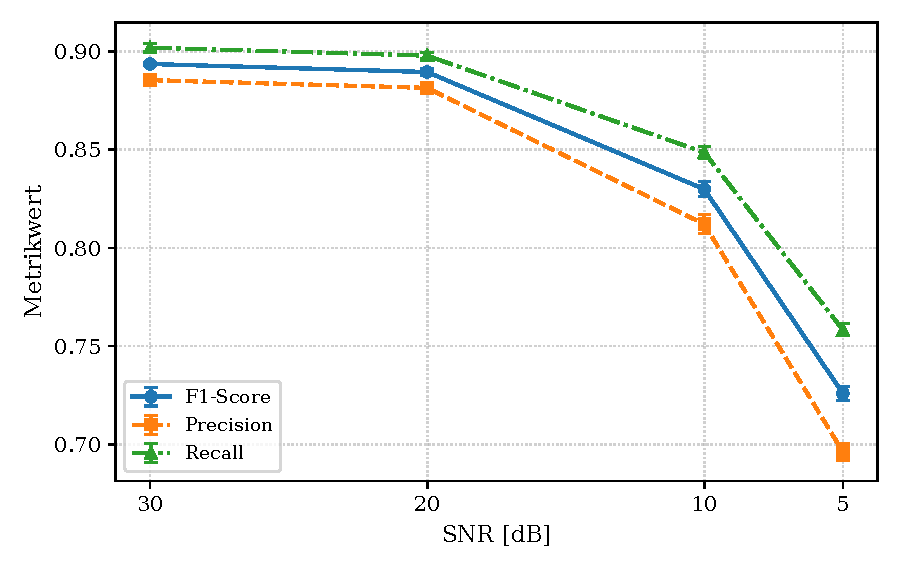
\includegraphics[width=0.85\textwidth]{snr_robustheit_plot.pdf}
	\caption{Precision, Recall und F1-Score des DDQN-Agenten über der SNR des AWGN-Kanals (30 bis 5\,dB). Marker: Mittelwert über drei Seeds, Fehlerbalken: $\pm$ eine Standardabweichung.}
	\label{fig:snr_robustheit}
\end{figure}

Der F1-Score fällt monoton von $0{,}8935$ bei 30\,dB über $0{,}8894$ (20\,dB) und $0{,}8298$ (10\,dB) auf $0{,}7260$ bei 5\,dB. Der Abfall verläuft nicht linear. Zwischen 30 und 20\,dB verliert der Agent nur $0{,}4$ Prozentpunkte, zwischen 10 und 5\,dB dagegen $10{,}4$. Das folgt aus dem Kanalmodell: Die Rauschvarianz je Merkmal beträgt $P_x/10^{\mathrm{SNR}/10}$, bei 30\,dB also $10^{-3}P_x$ und bei 5\,dB rund $0{,}32\,P_x$. Bei 20\,dB und darüber liegt die zusätzliche Varianz deutlich unter der intrinsischen Klassenstreuung von $\sigma=0{,}20$ je Merkmal und verändert die Überlappung der Klassen kaum. Bei 5\,dB überwiegt sie diese Streuung und verschmiert die Klassengrenze, die ohnehin nur über Mittelwertdifferenzen von $0{,}15$ bis $0{,}25$ je Merkmal definiert ist.

Die Streuung über die Seeds bleibt klein ($\sigma\le 0{,}0048$ bei allen Metriken) und wächst bei 10 und 5\,dB gegenüber 30\,dB auf das Zwei- bis Vierfache. Die Trainingsläufe konvergieren also reproduzierbar, bei starkem Rauschen reagiert die gelernte Entscheidungsgrenze jedoch empfindlicher auf die Initialisierung.

\subsection{Wirkung der asymmetrischen Reward-Funktion}
\label{sec:reward_recall}

Der Recall liegt auf allen vier SNR-Stufen über der Precision, am deutlichsten bei 5\,dB ($0{,}7583$ gegenüber $0{,}6963$). Das ist die direkte Folge der Belohnungsstruktur $R_{TP}=+1$, $R_{TN}=+0{,}5$, $R_{FP}=-1$, $R_{FN}=-2$. Da jeder Fluss eine Ein-Schritt-Episode ist, lernt die Q-Funktion den erwarteten Reward der Sofortentscheidung. Für die Angriffs-Posterior $p=P(\text{DDoS}\mid x)$ gilt
\begin{equation}
	Q(x,1)=p\cdot 1+(1-p)(-1)=2p-1,\qquad
	Q(x,0)=p\cdot(-2)+(1-p)\cdot 0{,}5=0{,}5-2{,}5\,p .
\end{equation}
Der Agent wählt \emph{DDoS}, sobald $Q(x,1)>Q(x,0)$ gilt, also für $p>1/3$. Ein symmetrisch bestrafender Klassifikator entscheidet dagegen bei $p>1/2$. Die Entscheidungsschwelle wandert damit zugunsten der Angriffsklasse. Der Agent akzeptiert mehr False Positives, um False Negatives zu vermeiden, und gibt Precision für Recall ab.

Das erklärt auch, warum bei sinkender SNR die Precision stärker einbricht als der Recall: Von 30 auf 5\,dB verliert die Precision $18{,}9$ Prozentpunkte, der Recall $14{,}4$. Mit zunehmender Unsicherheit der Posterior rutscht ein wachsender Anteil normaler Flüsse (Priorwahrscheinlichkeit $0{,}7$) über die abgesenkte Schwelle von $1/3$ und erzeugt zusätzliche Fehlalarme. Unter starkem Rauschen verhält sich der Agent konservativ im Sinne der Angriffserkennung, nicht im Sinne der Fehlalarmvermeidung.

\section{Vergleich mit klassischen Baselines}
\label{sec:baseline_vergleich}

Als Referenz dienen Random Forest (200 Bäume), SVM mit RBF-Kernel und ein MLP mit zwei verdeckten Schichten à 128 Neuronen. Sie verwenden dieselbe Datengenerierung und denselben AWGN-Kanal, dieselben Seeds und exakt dieselben Testflüsse je Seed und SNR-Stufe wie der DDQN. Trainiert wurden sie überwacht auf 20\,000 Flüssen mit pro Fluss gemischtem SNR. Tabelle~\ref{tab:f1_vergleich} stellt die F1-Scores gegenüber, Abbildung~\ref{fig:baseline_vergleich} zeigt den Verlauf.

\begin{table}[htbp]
	\centering
	\setlength{\tabcolsep}{4pt}
	\renewcommand{\arraystretch}{1.2}
	\caption{F1-Score von DDQN, Random Forest, SVM (RBF) und MLP je SNR-Stufe (Mittelwert $\pm$ Standardabweichung über drei Seeds). Fettdruck: höchster Mittelwert je Stufe.}
	\label{tab:f1_vergleich}
	\begin{tabular}{ccccc}
		\toprule
		\textbf{SNR [dB]} & \textbf{DDQN} & \textbf{Random Forest} & \textbf{SVM (RBF)} & \textbf{MLP} \\
		\midrule
		30 & $\mathbf{0{,}8935} \pm 0{,}0009$ & $0{,}8739 \pm 0{,}0032$ & $0{,}8857 \pm 0{,}0020$ & $0{,}8910 \pm 0{,}0010$ \\
		20 & $\mathbf{0{,}8894} \pm 0{,}0016$ & $0{,}8662 \pm 0{,}0026$ & $0{,}8795 \pm 0{,}0013$ & $0{,}8841 \pm 0{,}0022$ \\
		10 & $\mathbf{0{,}8298} \pm 0{,}0037$ & $0{,}8037 \pm 0{,}0031$ & $0{,}8211 \pm 0{,}0016$ & $0{,}8265 \pm 0{,}0064$ \\
		5  & $\mathbf{0{,}7260} \pm 0{,}0037$ & $0{,}6972 \pm 0{,}0060$ & $0{,}7097 \pm 0{,}0047$ & $0{,}7198 \pm 0{,}0003$ \\
		\bottomrule
	\end{tabular}
\end{table}

\begin{figure}[htbp]
	\centering
	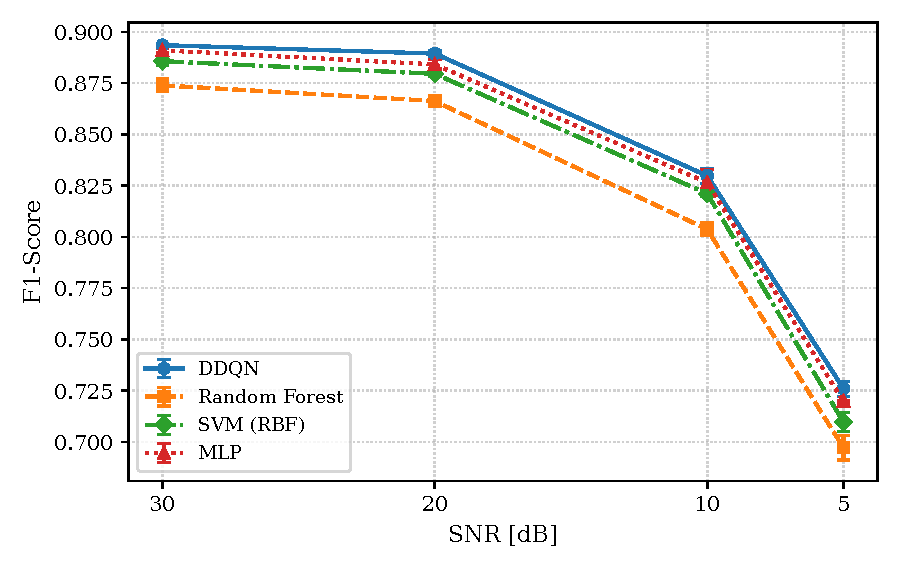
\includegraphics[width=0.85\textwidth]{baseline_vergleich_plot.pdf}
	\caption{F1-Score von DDQN, Random Forest, SVM (RBF) und MLP über der SNR des AWGN-Kanals. Marker: Mittelwert über drei Seeds, Fehlerbalken: $\pm$ eine Standardabweichung.}
	\label{fig:baseline_vergleich}
\end{figure}

Alle vier Verfahren zeigen denselben monotonen Abfall, und der DDQN erreicht auf jeder Stufe den höchsten mittleren F1-Score. Der Vorsprung ist allerdings klein. Gegenüber dem MLP, dem stärksten Baseline-Modell, beträgt er $0{,}25$ (30\,dB), $0{,}53$ (20\,dB), $0{,}33$ (10\,dB) und $0{,}62$ Prozentpunkte (5\,dB). Die SVM liegt zwischen $0{,}78$ und $1{,}63$, der Random Forest zwischen $1{,}96$ und $2{,}88$ Prozentpunkten zurück. Die Abstände zum MLP bewegen sich in der Größenordnung der Seed-Streuung, bei 10\,dB ($\sigma_{\mathrm{MLP}}=0{,}0064$) überlappen die Fehlerbalken. Mit drei Seeds lässt sich daraus keine statistische Signifikanz ableiten. Belastbar ist lediglich die Rangfolge DDQN $\gtrsim$ MLP $>$ SVM $>$ Random Forest, die auf allen vier Stufen identisch ausfällt.

Der DDQN erzielt seinen F1-Wert über einen anderen Arbeitspunkt als die Baselines. Beim Random Forest betragen Precision und Recall bei 30\,dB $0{,}9260$ und $0{,}8274$, beim DDQN $0{,}8853$ und $0{,}9018$. Die überwacht und ohne Kostengewichtung trainierten Baselines wählen die symmetrische Schwelle $p>1/2$ und landen entsprechend auf der Precision-Seite. Der F1-Score gewichtet beide Größen gleich und kann den Reward-getriebenen Arbeitspunkt des DDQN deshalb nur unvollständig bewerten. Unter der Kostenmatrix des Agenten, die einen verpassten Angriff doppelt so hoch bestraft wie einen Fehlalarm, fiele der Vorsprung gegenüber den Baselines voraussichtlich größer aus. Das wurde hier nicht gemessen.

Zwei Einschränkungen begrenzen die Aussagekraft des Vergleichs. Erstens sah der DDQN rund $6{,}4\cdot 10^{5}$ Trainingsflüsse (20\,000 Iterationen $\times$ 32), die Baselines nur $2\cdot 10^{4}$. Zweitens stammen alle Daten aus dem klassenbedingt gaußverteilten Generatormodell mit Angriffsanteil $0{,}3$. In einem solchen Modell erreicht schon ein kleines neuronales Netz eine nahezu Bayes-optimale Entscheidungsgrenze, was die geringen Unterschiede zwischen DDQN und MLP erklärt. Ob sich der Vorsprung auf realem Verkehr halten würde, bleibt offen.

\section{Robustheit nach RLA und ELA}
\label{sec:robustheit_rla_ela}

Tabelle~\ref{tab:rla_ela} wendet die Maße aus Abschnitt~\ref{sec:robustheitsmetriken} auf die mittleren F1-Scores an. Referenz ist jeweils die eigene Leistung des Modells bei 30\,dB.

\begin{table}[htbp]
	\centering
	\small
	\setlength{\tabcolsep}{4pt}
	\renewcommand{\arraystretch}{1.2}
	\caption{Relative Loss of Accuracy (RLA, in \%) und Equalized Loss of Accuracy (ELA) nach Sáez et al.\ \autocite{saezEvaluatingClassifierBehavior2016}, berechnet aus den mittleren F1-Scores über drei Seeds mit 30\,dB als Referenz. Kleinere Werte bedeuten höhere Robustheit.}
	\label{tab:rla_ela}
	\begin{tabular}{lccccccc}
		\toprule
		& \multicolumn{3}{c}{\textbf{RLA [\%]}} & \multicolumn{4}{c}{\textbf{ELA}} \\
		\cmidrule(lr){2-4}\cmidrule(lr){5-8}
		\textbf{Modell} & 20\,dB & 10\,dB & 5\,dB & 30\,dB & 20\,dB & 10\,dB & 5\,dB \\
		\midrule
		DDQN          & $\mathbf{0{,}46}$ & $\mathbf{7{,}13}$ & $\mathbf{18{,}75}$ & $\mathbf{0{,}119}$ & $\mathbf{0{,}124}$ & $\mathbf{0{,}191}$ & $\mathbf{0{,}307}$ \\
		MLP           & $0{,}77$ & $7{,}24$ & $19{,}21$ & $0{,}122$ & $0{,}130$ & $0{,}195$ & $0{,}315$ \\
		SVM (RBF)     & $0{,}70$ & $7{,}29$ & $19{,}87$ & $0{,}129$ & $0{,}136$ & $0{,}202$ & $0{,}328$ \\
		Random Forest & $0{,}88$ & $8{,}03$ & $20{,}22$ & $0{,}144$ & $0{,}153$ & $0{,}225$ & $0{,}347$ \\
		\bottomrule
	\end{tabular}
\end{table}

Die ELA ordnet die Modelle auf jeder Stufe gleich: DDQN vor MLP, SVM und Random Forest. Bei der RLA ist das nicht durchgehend so. Bei 20\,dB verliert die SVM relativ weniger als das MLP ($0{,}70$ gegenüber $0{,}77\,\%$), obwohl ihr F1-Score auf beiden Stufen niedriger liegt. Genau diesen Effekt korrigiert die ELA, indem sie den verbleibenden Fehler statt der Differenz bewertet.

Auffälliger als die Rangfolge ist die Spannweite. Bei 10\,dB liegen DDQN, MLP und SVM in der RLA nur $0{,}16$ Prozentpunkte auseinander, der Random Forest $0{,}9$ Prozentpunkte hinter dem DDQN. Bei 5\,dB verlieren alle vier Modelle zwischen $18{,}8$ und $20{,}2\,\%$ ihrer Ausgangsleistung. Der Großteil des Verlusts ist also nicht modellbedingt, sondern folgt aus der Klassenüberlappung des Kanals: Die Bayes-Fehlerwahrscheinlichkeit steigt im selben Intervall von $6{,}9$ auf $18{,}7\,\%$ (Tabelle~\ref{tab:klassenueberlappung}). Modellbedingt ist nur die Differenz zwischen den Verfahren, bei 5\,dB rund $1{,}5$ Prozentpunkte RLA zwischen DDQN und Random Forest. Wie beim F1-Vergleich gilt: Mit drei Seeds ist dieser Abstand nicht als signifikant nachgewiesen.

\section{Einordnung in die Literatur}
\label{sec:ergebnisse_literatur}

\paragraph{Random Forest als schwächste Baseline.} Arjoune et al. finden für die Jamming-Erkennung in der Accuracy die Rangfolge Random Forest ($96{,}6\,\%$) vor neuronalem Netz ($94{,}4\,\%$) und SVM \autocite{arjouneNovelJammingAttacks2020}. Hier fällt sie umgekehrt aus. Zwei Unterschiede erklären das. Bei Arjoune et al. ist die Kanalverschlechterung selbst das Ereignis, das die vier Linkqualitätsmerkmale (Bad Packet Ratio, Packet Delivery Ratio, Received Signal Strength, Clear Channel Assessment) anzeigen. Hier ist das Rauschen eine Störung, die alle acht Flussmerkmale überlagert und keine Information über die Klasse trägt. Der zweite Grund liegt im Generatormodell. Bei gleicher Kovarianz beider Klassen ist der Logarithmus des Likelihood-Verhältnisses linear in $\mathbf{y}$, die Bayes-optimale Grenze also eine Hyperebene mit der Normalen $\boldsymbol{\Sigma}^{-1}\Delta\boldsymbol{\mu}$. Weil $\boldsymbol{\Sigma}$ vom SNR abhängt, ändert sich ihre Richtung über die gemischten Trainingsstufen nur geringfügig, die Grenze bleibt nahezu linear und liegt schräg zu den Koordinatenachsen. Q-Netz, MLP und RBF-SVM bilden eine solche Fläche direkt ab. Ein Random Forest muss sie aus achsenparallelen Stufen zusammensetzen, und jede dieser Stufen reagiert auf Rauschen nahe ihrer Schwelle, wie es Zhu und Wu für Entscheidungsbäume beschreiben \autocite{zhuClassNoiseVs2004}.

\paragraph{DDQN und MLP.} Q-Netz und MLP haben dieselbe Struktur $8\to128\to128$ mit ReLU und unterscheiden sich im Lernziel. Das MLP schätzt über die Kreuzentropie die Posterior $p$ und entscheidet bei $p>1/2$. Das Q-Netz regressiert den erwarteten Reward und entscheidet damit bei $p>1/3$ (Abschnitt~\ref{sec:reward_recall}). Die fast gleichen ELA-Werte passen dazu: Beide lernen eine vergleichbar gute Repräsentation, der F1-Unterschied stammt überwiegend aus dem Arbeitspunkt. Zhang et al. zeigen, dass MLP-basierte NIDS unter gezielter Manipulation zeitbasierter Merkmale umgangen werden können \autocite{zhangAdversarialAttacksDeep2022}. Dieser Befund betrifft das Q-Netz gleichermaßen, da es architektonisch ein MLP ist.

\paragraph{Stochastische gegenüber gezielter Störung.} Die gemessene Robustheit gilt nur für AWGN. Merzouk et al. zeigen, dass die Accuracy eines DQN-Detektors unter FGSM von $84{,}81$ auf $66{,}87\,\%$ fällt \autocite{merzoukEvadingDeepReinforcement2022}. Der Unterschied lässt sich am Generatormodell abschätzen. In weißen Koordinaten, in denen die Klassenstreuung isotrop ist, entscheidet nur die Komponente der Störung entlang der Diskriminanten. Näherungsweise isotropes Rauschen legt im Mittel nur den Anteil $1/8$ seiner Leistung in diese Richtung, eine gezielte Störung ihre gesamte. Bei gleicher Leistung ist der gezielte Angriff damit um etwa den Faktor $\sqrt{8}\approx2{,}8$ in der Amplitude wirksamer. Ein gutes Ergebnis unter AWGN ist deshalb kein Beleg für adversariale Robustheit.

\section{Zusammenfassung}
\label{sec:ergebnisse_zusammenfassung}

Der DDQN-Agent erreicht bei 30\,dB einen F1-Score von $0{,}8935$ und hält bei 10\,dB noch $0{,}8298$. Bei 5\,dB fällt er auf $0{,}7260$. Der Recall übertrifft die Precision auf jeder Stufe, weil die Reward-Matrix die Entscheidungsschwelle von $p=1/2$ auf $p=1/3$ senkt. Gegenüber Random Forest, SVM und MLP liegt der DDQN auf allen vier SNR-Stufen vorn, der Abstand zum MLP bleibt jedoch unter einem Prozentpunkt und innerhalb weniger Standardabweichungen. Nach der ELA bleibt der DDQN auf allen Stufen das robusteste Verfahren ($0{,}307$ bei 5\,dB gegenüber $0{,}347$ beim Random Forest). Der größte Teil des Leistungsverlusts geht jedoch auf die wachsende Klassenüberlappung zurück und trifft alle Modelle ähnlich. Die Ergebnisse belegen die Robustheit des Ansatzes bis etwa 10\,dB, und zwar gegenüber stochastischem Rauschen, nicht gegenüber gezielten Angriffen. Einen klaren Überlegenheitsnachweis gegenüber überwacht trainierten Klassifikatoren liefern sie nicht.

\chapter{Fazit und Ausblick}
\label{chap:fazit}

\section{Zusammenfassung und Schlussfolgerung}
\label{sec:fazit_zusammenfassung}

Die vorliegende Arbeit hat die Erkennung von DDoS-ähnlichen Angriffsmustern als sequenzielles Entscheidungsproblem in einer dynamischen, verrauschten Netzwerkumgebung modelliert und mit einem Double Deep Q-Network (DDQN) umgesetzt. Ausgangspunkt war die in Kapitel~\ref{chap:einleitung} formulierte Fragestellung, inwieweit KI-basierte Verfahren unter realitätsnahen Störbedingungen eine belastbare Angriffserkennung ermöglichen. Auf Basis der in Kapitel~\ref{chap:grundlagen} und Kapitel~\ref{chap:related_work} diskutierten methodischen Grundlagen wurde in Kapitel~\ref{chap:datensatz} eine konsistente Datenpipeline aufgebaut und in Kapitel~\ref{chap:implementierung} eine reproduzierbare RL-Umgebung mit AWGN-Modellierung implementiert. Kapitel~\ref{chap:evaluierung} hat das Evaluationsprotokoll und die Metriken festgelegt, Kapitel~\ref{chap:ergebnisse} die Leistungsfähigkeit des Ansatzes im Vergleich mit den Baselines empirisch quantifiziert.

Die Ergebnisse zeigen, dass der Double-DQN-Agent (DDQN) bei 30\,dB einen F1-Score von $0{,}8935$ erreicht (Precision $0{,}8853$, Recall $0{,}9018$). Gegenüber Random Forest, SVM und MLP liegt er auf allen vier SNR-Stufen vorn. Der Vorsprung gegenüber dem MLP beträgt allerdings nur $0{,}25$ bis $0{,}62$ Prozentpunkte und bewegt sich in der Größenordnung der Seed-Streuung. Belastbar ist die Rangfolge DDQN $\gtrsim$ MLP $>$ SVM $>$ Random Forest, nicht ein signifikanter Vorsprung. Die Equalized Loss of Accuracy nach Sáez et al. bestätigt diese Rangfolge auf allen SNR-Stufen \autocite{saezEvaluatingClassifierBehavior2016}. Bei 5\,dB verlieren alle vier Verfahren zwischen $18{,}8$ und $20{,}2\,\%$ ihres F1-Scores. Der Verlust folgt damit überwiegend aus der Klassenüberlappung des Kanals, nicht aus dem Modell. Dass der Random Forest hier zurückliegt, während er in der Jamming-Erkennung von Arjoune et al. vorn liegt \autocite{arjouneNovelJammingAttacks2020}, erklärt sich aus der nahezu linearen, schräg im Merkmalsraum liegenden Bayes-Grenze des Generatormodells (Abschnitt~\ref{sec:ergebnisse_literatur}).

Über die untersuchten SNR-Stufen von 30\,dB bis 5\,dB fällt der F1-Score monoton ab, zunächst moderat von $0{,}8935$ auf $0{,}8298$ bei 10\,dB, bei 5\,dB dann auf $0{,}7260$. Der Agent bleibt damit bis etwa 10\,dB operationell nutzbar. Der Recall liegt auf jeder Stufe über der Precision, weil die asymmetrische Reward-Matrix ($R_{FN}=-2$, $R_{FP}=-1$) die Entscheidungsschwelle auf eine Angriffs-Posterior von $1/3$ senkt. Bei sinkendem SNR bricht deshalb die Precision stärker ein als der Recall. Für den Netzbetrieb heißt das: Unter schlechten Kanalbedingungen steigt die Zahl der Fehlalarme schneller als die Zahl verpasster Angriffe.

Im Gesamtfazit bestätigt die Arbeit die Eignung des RL-basierten Ansatzes für die adaptive DDoS-Erkennung in dynamischen Kommunikationsnetzen. Die Kombination aus sequenzieller Entscheidungslogik, Experience Replay, Zielnetzwerk und rauschbehafteter Umweltsimulation liefert einen methodischen Mehrwert gegenüber rein statischen Klassifikationsverfahren. Zugleich bleiben Grenzen sichtbar: Die Aussagekraft ist an das gewählte Simulationsdesign, die betrachteten Merkmale und die Abdeckung der Datensätze gebunden. Für eine weitergehende Generalisierung sind daher zusätzliche Untersuchungen auf heterogeneren Lastprofilen, realen Traffic-Spuren und erweiterten Angriffstypen notwendig \autocite{balaAITechniquesIoTbased2024, kumarComprehensiveReviewVulnerabilities2024}.

\section{Ausblick und Forschungsperspektiven}
\label{sec:fazit_ausblick}

Aus den gewonnenen Befunden ergeben sich mehrere fundierte Forschungsperspektiven für zukünftige Arbeiten:

\begin{enumerate}
    \item \textbf{Validierung auf den Originaldatensätzen:} Die Experimente dieser Arbeit nutzen ein parametrisches Flussmodell, dessen Merkmalsstruktur sich an DDoS-AT-2022 \autocite{mittalDDoSAT2022DistributedDenial2023} und IoT-DH \autocite{saifIoTDHDatasetClassification2024} orientiert (Abschnitt~\ref{sec:generatormodell}). Der nächste Schritt ist die Wiederholung von Training und Test auf den Originaldaten beider Datensätze, mit einem getrennten Validierungs-Split, einem AWGN-Kanal auf den realen Merkmalen und denselben Baselines. Erst dieser Vergleich zeigt, ob die Rangfolge und die SNR-Robustheit auf realem Verkehr bestehen bleiben. Dabei lässt sich zugleich prüfen, ob die Reward-getriebene Verschiebung zum Recall auch bei den realen Klassenverhältnissen (z.\,B. rund $37\,\%$ Angriffsanteil in IoT-DH) erhalten bleibt.
    \item \textbf{Erweiterung auf komplexe Netzwerktopologien:} Der Ansatz sollte auf komplexere Topologien mit hierarchischen Segmenten, variabler Linkqualität und verteilten Kontrollinstanzen übertragen werden, um die Skalierbarkeit in realen Betreiberumgebungen zu validieren.
    \item \textbf{Einsatz fortgeschrittener RL-Architekturen:} Zur Steigerung der Lernstabilität und Sample-Effizienz bietet sich \textit{Prioritized Experience Replay} an. Sinnvoll wird der Bootstrapping-Anteil des DDQN erst bei mehrschrittigen Formulierungen, etwa wenn der Agent Verkehrsfenster sequenziell beobachtet und Gegenmaßnahmen steuert.
    \item \textbf{Multi-Agenten-Systeme:} Die Untersuchung kooperativer Multi-Agenten-Architekturen, bei denen spezialisierte Agenten verteilt für Erkennung, Priorisierung und automatisierte Gegenmaßnahmen zusammenwirken, verspricht eine weitere Reduktion der Reaktionszeiten.
    \item \textbf{Gezielte Störungen und robustes Training:} Die gemessene Robustheit gilt nur für stochastisches AWGN. Der nächste Test ist ein Angriff mit FGSM und BIM auf denselben Agenten, wie ihn Merzouk et al. für einen DRL-Detektor durchgeführt haben \autocite{merzoukEvadingDeepReinforcement2022}. Als Gegenmaßnahme bietet sich der Regularisierer aus dem SA-MDP-Rahmen von Zhang et al. an, der die Änderung der gewählten Aktion innerhalb einer $\varepsilon$-Umgebung der Beobachtung begrenzt \autocite{zhangRobustDeepReinforcement2020}. Ran et al. setzen eine gegen gestörte Zustandsbeobachtungen robust trainierte DQN bereits zur Erkennung von False-Data-Injection-Angriffen in Stromnetzen ein \autocite{ranRobustDataDrivenAdversarial2024}. Ob sich der Ansatz auf Flussmerkmale übertragen lässt, ist offen.
    \item \textbf{Betriebskennzahlen und Erklärbarkeit:} Die Leistungsanalyse sollte um Latenz, Ressourcenverbrauch und Verfahren der \textit{Explainable AI} (XAI) ergänzt werden.
\end{enumerate}

In der Gesamtschau liefert die Arbeit damit einen konsistenten Beitrag zur KI-gestützten Angriffserkennung: Sie verbindet theoretische Fundierung, reproduzierbare Implementierung und empirische Robustheitsanalyse zu einem geschlossenen methodischen Rahmen. Die Ergebnisse unterstützen die zentrale Arbeitshypothese, dass DDQN-basierte Verfahren bei geeigneter Modellierung und Evaluation eine leistungsfähige und zugleich ausbaufähige Grundlage für adaptive DDoS-Abwehr in modernen Kommunikationsnetzen darstellen.

% ---------------------------------------------------------------
% Literaturverzeichnis
% ---------------------------------------------------------------
\printbibliography[heading=bibintoc, title={Literaturverzeichnis}]

\end{document}